\documentclass[tikz,crop,convert={density=200,outext=.png},border=0.4cm]{standalone}

\usetikzlibrary{backgrounds}
\usepackage{pgfplots}
\usepackage{amsmath}
\usetikzlibrary{arrows.meta}
\usepackage{physics}
\usepackage{xcolor}
\usepgfplotslibrary{fillbetween}
% Define the colours of the linear model
\definecolor{lin_1}{RGB}{0,68,27}
\definecolor{lin_2}{RGB}{0,109,44}
\definecolor{lin_3}{RGB}{35,139,69}
% Define the colours of the cubic model
\definecolor{cube_1}{RGB}{103,0,31}
\definecolor{cube_2}{RGB}{152,0,67}
\definecolor{cube_3}{RGB}{206,18,86}


\pgfplotsset{compat=newest,
    %width=6cm,
    %height=3cm,
    scale only axis=true,
    max space between ticks=25pt,
    try min ticks=5,
    every axis/.style={
        axis y line=middle,
        axis x line=middle,
        % axis line style={thick,<->,>=latex, shorten >=-.3cm}
        axis line style={thick,<->,>=latex, shorten >=-.3cm, shorten <=-.3cm}
    },
    every axis plot/.append style={thick},
    tick style={black, thick},
}
\tikzset{
    semithick/.style={line width=0.8pt},
}
\usepgfplotslibrary{groupplots}
\usepgfplotslibrary{dateplot}
%\pgfplotsset{compat=1.16}
% Document begins
\begin{document}
%=========================================================================================================
% FIGURE LINE
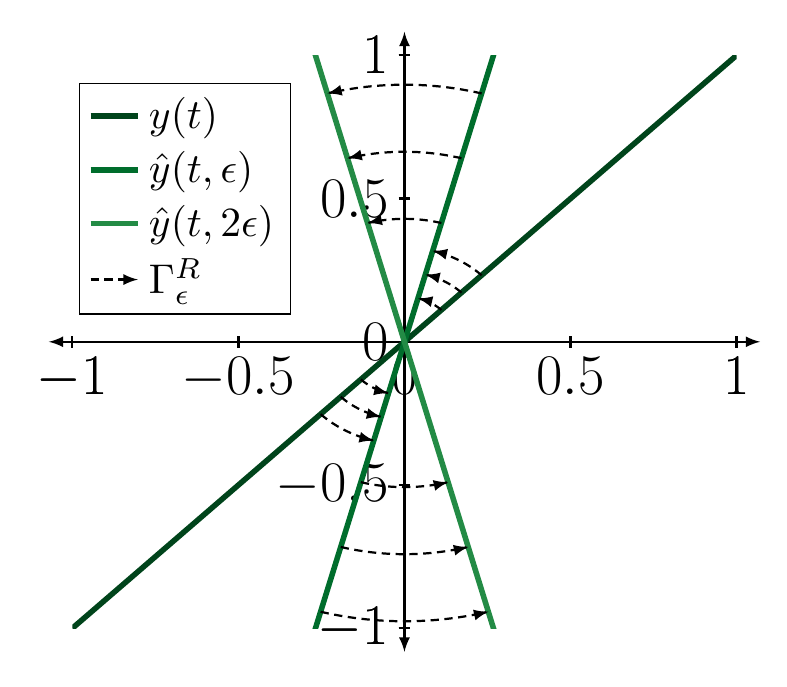
\begin{tikzpicture}
  % The axis of the plot
  \begin{axis}[
    x label style={at={(axis description cs:0.5,-0.15)},anchor=north},
    y label style={at={(axis description cs:-0.15,0.55)},rotate=90,anchor=south,align={center}},    
    legend style={at={(axis description cs:0.01,0.75)},anchor=west,nodes={scale=1.5, transform shape}},
    ymin = -1,
    ymax = 1,
    xmin=-1,
    xmax = 1,
    ytick = {-1,-0.5,...,1},
    xtick = {-1,-0.5,...,1},
    axis x line*=middle,
    extra x ticks={0,-1,1},
    extra y ticks = {0,-1,1},
    grid style=dashed,
    label style={font=\huge},
    tick label style={font=\huge},
    legend cell align={left},    
]
\addplot[
color=lin_1,line width=2pt,
]
coordinates {%
(-1.0,-1.0)
(-0.9797979797979798,-0.9797979797979798)
(-0.9595959595959596,-0.9595959595959596)
(-0.9393939393939394,-0.9393939393939394)
(-0.9191919191919192,-0.9191919191919192)
(-0.898989898989899,-0.898989898989899)
(-0.8787878787878788,-0.8787878787878788)
(-0.8585858585858586,-0.8585858585858586)
(-0.8383838383838383,-0.8383838383838383)
(-0.8181818181818181,-0.8181818181818181)
(-0.797979797979798,-0.797979797979798)
(-0.7777777777777778,-0.7777777777777778)
(-0.7575757575757576,-0.7575757575757576)
(-0.7373737373737373,-0.7373737373737373)
(-0.7171717171717171,-0.7171717171717171)
(-0.696969696969697,-0.696969696969697)
(-0.6767676767676767,-0.6767676767676767)
(-0.6565656565656566,-0.6565656565656566)
(-0.6363636363636364,-0.6363636363636364)
(-0.6161616161616161,-0.6161616161616161)
(-0.5959595959595959,-0.5959595959595959)
(-0.5757575757575757,-0.5757575757575757)
(-0.5555555555555556,-0.5555555555555556)
(-0.5353535353535352,-0.5353535353535352)
(-0.5151515151515151,-0.5151515151515151)
(-0.4949494949494949,-0.4949494949494949)
(-0.4747474747474747,-0.4747474747474747)
(-0.4545454545454545,-0.4545454545454545)
(-0.43434343434343425,-0.43434343434343425)
(-0.41414141414141414,-0.41414141414141414)
(-0.3939393939393939,-0.3939393939393939)
(-0.3737373737373737,-0.3737373737373737)
(-0.3535353535353535,-0.3535353535353535)
(-0.33333333333333326,-0.33333333333333326)
(-0.31313131313131304,-0.31313131313131304)
(-0.2929292929292928,-0.2929292929292928)
(-0.2727272727272727,-0.2727272727272727)
(-0.2525252525252525,-0.2525252525252525)
(-0.23232323232323226,-0.23232323232323226)
(-0.21212121212121204,-0.21212121212121204)
(-0.19191919191919182,-0.19191919191919182)
(-0.1717171717171716,-0.1717171717171716)
(-0.1515151515151515,-0.1515151515151515)
(-0.13131313131313127,-0.13131313131313127)
(-0.11111111111111105,-0.11111111111111105)
(-0.09090909090909083,-0.09090909090909083)
(-0.07070707070707061,-0.07070707070707061)
(-0.050505050505050386,-0.050505050505050386)
(-0.030303030303030276,-0.030303030303030276)
(-0.010101010101010055,-0.010101010101010055)
(0.010101010101010166,0.010101010101010166)
(0.030303030303030498,0.030303030303030498)
(0.05050505050505061,0.05050505050505061)
(0.07070707070707072,0.07070707070707072)
(0.09090909090909105,0.09090909090909105)
(0.11111111111111116,0.11111111111111116)
(0.1313131313131315,0.1313131313131315)
(0.1515151515151516,0.1515151515151516)
(0.1717171717171717,0.1717171717171717)
(0.19191919191919204,0.19191919191919204)
(0.21212121212121215,0.21212121212121215)
(0.2323232323232325,0.2323232323232325)
(0.2525252525252526,0.2525252525252526)
(0.27272727272727293,0.27272727272727293)
(0.29292929292929304,0.29292929292929304)
(0.31313131313131315,0.31313131313131315)
(0.3333333333333335,0.3333333333333335)
(0.3535353535353536,0.3535353535353536)
(0.3737373737373739,0.3737373737373739)
(0.39393939393939403,0.39393939393939403)
(0.41414141414141437,0.41414141414141437)
(0.4343434343434345,0.4343434343434345)
(0.4545454545454546,0.4545454545454546)
(0.4747474747474749,0.4747474747474749)
(0.49494949494949503,0.49494949494949503)
(0.5151515151515154,0.5151515151515154)
(0.5353535353535355,0.5353535353535355)
(0.5555555555555556,0.5555555555555556)
(0.5757575757575759,0.5757575757575759)
(0.595959595959596,0.595959595959596)
(0.6161616161616164,0.6161616161616164)
(0.6363636363636365,0.6363636363636365)
(0.6565656565656568,0.6565656565656568)
(0.6767676767676769,0.6767676767676769)
(0.696969696969697,0.696969696969697)
(0.7171717171717173,0.7171717171717173)
(0.7373737373737375,0.7373737373737375)
(0.7575757575757578,0.7575757575757578)
(0.7777777777777779,0.7777777777777779)
(0.7979797979797982,0.7979797979797982)
(0.8181818181818183,0.8181818181818183)
(0.8383838383838385,0.8383838383838385)
(0.8585858585858588,0.8585858585858588)
(0.8787878787878789,0.8787878787878789)
(0.8989898989898992,0.8989898989898992)
(0.9191919191919193,0.9191919191919193)
(0.9393939393939394,0.9393939393939394)
(0.9595959595959598,0.9595959595959598)
(0.9797979797979799,0.9797979797979799)
(1.0,1.0)
};
\addlegendentry{$y(t)$}
\addplot[
color=lin_2,line width=2pt,
]
coordinates {%
(-1.0,-3.732050807568876)
(-0.9797979797979798,-3.6566558417594037)
(-0.9595959595959596,-3.581260875949931)
(-0.9393939393939394,-3.5058659101404595)
(-0.9191919191919192,-3.430470944330987)
(-0.898989898989899,-3.3550759785215147)
(-0.8787878787878788,-3.2796810127120426)
(-0.8585858585858586,-3.20428604690257)
(-0.8383838383838383,-3.128891081093098)
(-0.8181818181818181,-3.0534961152836253)
(-0.797979797979798,-2.9781011494741536)
(-0.7777777777777778,-2.9027061836646815)
(-0.7575757575757576,-2.827311217855209)
(-0.7373737373737373,-2.7519162520457368)
(-0.7171717171717171,-2.676521286236264)
(-0.696969696969697,-2.6011263204267925)
(-0.6767676767676767,-2.52573135461732)
(-0.6565656565656566,-2.4503363888078478)
(-0.6363636363636364,-2.3749414229983756)
(-0.6161616161616161,-2.299546457188903)
(-0.5959595959595959,-2.224151491379431)
(-0.5757575757575757,-2.1487565255699588)
(-0.5555555555555556,-2.0733615597604866)
(-0.5353535353535352,-1.997966593951014)
(-0.5151515151515151,-1.9225716281415421)
(-0.4949494949494949,-1.8471766623320698)
(-0.4747474747474747,-1.7717816965225974)
(-0.4545454545454545,-1.696386730713125)
(-0.43434343434343425,-1.6209917649036527)
(-0.41414141414141414,-1.545596799094181)
(-0.3939393939393939,-1.4702018332847087)
(-0.3737373737373737,-1.3948068674752363)
(-0.3535353535353535,-1.319411901665764)
(-0.33333333333333326,-1.2440169358562916)
(-0.31313131313131304,-1.1686219700468194)
(-0.2929292929292928,-1.093227004237347)
(-0.2727272727272727,-1.0178320384278752)
(-0.2525252525252525,-0.9424370726184028)
(-0.23232323232323226,-0.8670421068089306)
(-0.21212121212121204,-0.7916471409994582)
(-0.19191919191919182,-0.716252175189986)
(-0.1717171717171716,-0.6408572093805136)
(-0.1515151515151515,-0.5654622435710417)
(-0.13131313131313127,-0.4900672777615694)
(-0.11111111111111105,-0.4146723119520971)
(-0.09090909090909083,-0.3392773461426248)
(-0.07070707070707061,-0.2638823803331525)
(-0.050505050505050386,-0.18848741452368015)
(-0.030303030303030276,-0.11309244871420826)
(-0.010101010101010055,-0.03769748290473595)
(0.010101010101010166,0.03769748290473636)
(0.030303030303030498,0.11309244871420909)
(0.05050505050505061,0.18848741452368098)
(0.07070707070707072,0.26388238033315287)
(0.09090909090909105,0.3392773461426256)
(0.11111111111111116,0.4146723119520975)
(0.1313131313131315,0.4900672777615702)
(0.1515151515151516,0.5654622435710421)
(0.1717171717171717,0.640857209380514)
(0.19191919191919204,0.7162521751899867)
(0.21212121212121215,0.7916471409994587)
(0.2323232323232325,0.8670421068089313)
(0.2525252525252526,0.9424370726184033)
(0.27272727272727293,1.017832038427876)
(0.29292929292929304,1.093227004237348)
(0.31313131313131315,1.16862197004682)
(0.3333333333333335,1.2440169358562925)
(0.3535353535353536,1.3194119016657644)
(0.3737373737373739,1.3948068674752372)
(0.39393939393939403,1.470201833284709)
(0.41414141414141437,1.5455967990941817)
(0.4343434343434345,1.6209917649036536)
(0.4545454545454546,1.6963867307131255)
(0.4747474747474749,1.7717816965225983)
(0.49494949494949503,1.8471766623320702)
(0.5151515151515154,1.9225716281415428)
(0.5353535353535355,1.9979665939510147)
(0.5555555555555556,2.0733615597604866)
(0.5757575757575759,2.148756525569959)
(0.595959595959596,2.2241514913794314)
(0.6161616161616164,2.299546457188904)
(0.6363636363636365,2.374941422998376)
(0.6565656565656568,2.4503363888078487)
(0.6767676767676769,2.5257313546173203)
(0.696969696969697,2.6011263204267925)
(0.7171717171717173,2.676521286236265)
(0.7373737373737375,2.751916252045737)
(0.7575757575757578,2.82731121785521)
(0.7777777777777779,2.9027061836646815)
(0.7979797979797982,2.9781011494741545)
(0.8181818181818183,3.053496115283626)
(0.8383838383838385,3.1288910810930983)
(0.8585858585858588,3.204286046902571)
(0.8787878787878789,3.279681012712043)
(0.8989898989898992,3.3550759785215156)
(0.9191919191919193,3.4304709443309873)
(0.9393939393939394,3.5058659101404595)
(0.9595959595959598,3.581260875949932)
(0.9797979797979799,3.656655841759404)
(1.0,3.732050807568876)
};
\addlegendentry{$\hat{y}(t,\epsilon)$}
\addplot[
color=lin_3,line width=2pt,
]
coordinates {%
(-1.0,3.7320508075688794)
(-0.9797979797979798,3.656655841759407)
(-0.9595959595959596,3.5812608759499347)
(-0.9393939393939394,3.5058659101404626)
(-0.9191919191919192,3.4304709443309904)
(-0.898989898989899,3.355075978521518)
(-0.8787878787878788,3.2796810127120457)
(-0.8585858585858586,3.204286046902573)
(-0.8383838383838383,3.1288910810931005)
(-0.8181818181818181,3.0534961152836284)
(-0.797979797979798,2.9781011494741563)
(-0.7777777777777778,2.902706183664684)
(-0.7575757575757576,2.8273112178552116)
(-0.7373737373737373,2.7519162520457394)
(-0.7171717171717171,2.676521286236267)
(-0.696969696969697,2.6011263204267947)
(-0.6767676767676767,2.525731354617322)
(-0.6565656565656566,2.45033638880785)
(-0.6363636363636364,2.374941422998378)
(-0.6161616161616161,2.2995464571889053)
(-0.5959595959595959,2.224151491379433)
(-0.5757575757575757,2.1487565255699606)
(-0.5555555555555556,2.073361559760489)
(-0.5353535353535352,1.9979665939510158)
(-0.5151515151515151,1.922571628141544)
(-0.4949494949494949,1.8471766623320716)
(-0.4747474747474747,1.7717816965225992)
(-0.4545454545454545,1.6963867307131268)
(-0.43434343434343425,1.6209917649036543)
(-0.41414141414141414,1.5455967990941823)
(-0.3939393939393939,1.47020183328471)
(-0.3737373737373737,1.3948068674752376)
(-0.3535353535353535,1.3194119016657653)
(-0.33333333333333326,1.244016935856293)
(-0.31313131313131304,1.1686219700468206)
(-0.2929292929292928,1.0932270042373482)
(-0.2727272727272727,1.017832038427876)
(-0.2525252525252525,0.9424370726184037)
(-0.23232323232323226,0.8670421068089313)
(-0.21212121212121204,0.791647140999459)
(-0.19191919191919182,0.7162521751899866)
(-0.1717171717171716,0.6408572093805143)
(-0.1515151515151515,0.5654622435710422)
(-0.13131313131313127,0.4900672777615699)
(-0.11111111111111105,0.41467231195209747)
(-0.09090909090909083,0.3392773461426251)
(-0.07070707070707061,0.2638823803331527)
(-0.050505050505050386,0.18848741452368034)
(-0.030303030303030276,0.11309244871420837)
(-0.010101010101010055,0.037697482904735985)
(0.010101010101010166,-0.0376974829047364)
(0.030303030303030498,-0.11309244871420919)
(0.05050505050505061,-0.18848741452368117)
(0.07070707070707072,-0.26388238033315314)
(0.09090909090909105,-0.33927734614262595)
(0.11111111111111116,-0.4146723119520979)
(0.1313131313131315,-0.4900672777615707)
(0.1515151515151516,-0.5654622435710427)
(0.1717171717171717,-0.6408572093805146)
(0.19191919191919204,-0.7162521751899874)
(0.21212121212121215,-0.7916471409994594)
(0.2323232323232325,-0.8670421068089322)
(0.2525252525252526,-0.9424370726184041)
(0.27272727272727293,-1.017832038427877)
(0.29292929292929304,-1.0932270042373489)
(0.31313131313131315,-1.168621970046821)
(0.3333333333333335,-1.2440169358562936)
(0.3535353535353536,-1.3194119016657657)
(0.3737373737373739,-1.3948068674752385)
(0.39393939393939403,-1.4702018332847104)
(0.41414141414141437,-1.5455967990941832)
(0.4343434343434345,-1.6209917649036552)
(0.4545454545454546,-1.696386730713127)
(0.4747474747474749,-1.7717816965225999)
(0.49494949494949503,-1.847176662332072)
(0.5151515151515154,-1.9225716281415448)
(0.5353535353535355,-1.9979665939510167)
(0.5555555555555556,-2.073361559760489)
(0.5757575757575759,-2.1487565255699614)
(0.595959595959596,-2.2241514913794336)
(0.6161616161616164,-2.299546457188906)
(0.6363636363636365,-2.3749414229983783)
(0.6565656565656568,-2.450336388807851)
(0.6767676767676769,-2.525731354617323)
(0.696969696969697,-2.6011263204267947)
(0.7171717171717173,-2.6765212862362677)
(0.7373737373737375,-2.75191625204574)
(0.7575757575757578,-2.8273112178552124)
(0.7777777777777779,-2.9027061836646846)
(0.7979797979797982,-2.978101149474157)
(0.8181818181818183,-3.0534961152836293)
(0.8383838383838385,-3.128891081093101)
(0.8585858585858588,-3.204286046902574)
(0.8787878787878789,-3.279681012712046)
(0.8989898989898992,-3.3550759785215187)
(0.9191919191919193,-3.430470944330991)
(0.9393939393939394,-3.5058659101404626)
(0.9595959595959598,-3.5812608759499356)
(0.9797979797979799,-3.6566558417594073)
(1.0,-3.7320508075688794)
};
\addlegendentry{$\hat{y}(t,2\epsilon)$}
\addplot[
color=black,->,>=latex,densely dashed
]
coordinates {%
(-0.2525252525252525,-0.2525252525252525)
(-0.2507321635199357,-0.2543056989186387)
(-0.24892652167322896,-0.25607341356250274)
(-0.24710841738412773,-0.25782830795666484)
(-0.2452779416755564,-0.25957029424278777)
(-0.24343518618981141,-0.2612992852087753)
(-0.24158024318397298,-0.2630151942931388)
(-0.23971320552528647,-0.2647179355893304)
(-0.23783416668651278,-0.26640742385004423)
(-0.23594322074124902,-0.2680835744914845)
(-0.23404046235921838,-0.26974630359759955)
(-0.2321259868015308,-0.2713955279242836)
(-0.23019988991591342,-0.2730311649035443)
(-0.2282622681319123,-0.27465313264763613)
(-0.2263132184560647,-0.27626134995316054)
(-0.224352838467042,-0.2778557363051309)
(-0.22238122631076512,-0.2794362118810039)
(-0.2203984806954905,-0.2810026975546758)
(-0.2184047008868682,-0.2825551149004433)
(-0.21639998670297245,-0.2840933861969307)
(-0.2143844385093041,-0.28561743443098053)
(-0.2123581572137661,-0.2871271833015092)
(-0.21032124426161114,-0.2886225572233272)
(-0.2082738016303632,-0.290103481330923)
(-0.20621593182471193,-0.29156988148221147)
(-0.2041477378713808,-0.29302168426224545)
(-0.20206932331396904,-0.2944588169868916)
(-0.19998079220776785,-0.295881207706469)
(-0.19788224911455082,-0.2972887852093515)
(-0.19577379909733905,-0.2986814790255328)
(-0.19365554771514135,-0.3000592194301546)
(-0.1915276010176693,-0.3014219374469973)
(-0.1893900655400279,-0.30276956485193324)
(-0.18724304829738206,-0.30410203417634235)
(-0.1850866567795988,-0.3054192787104902)
(-0.18292099894586572,-0.30672123250686717)
(-0.18074618321928626,-0.3080078303834909)
(-0.17856231848145138,-0.3092790079271689)
(-0.17636951406698848,-0.3105347014967239)
(-0.1741678797580875,-0.3117748482261798)
(-0.17195752577900486,-0.31299938602790894)
(-0.16973856279054506,-0.3142082535957406)
(-0.1675111018845203,-0.3154013904080306)
(-0.16527525457818903,-0.31657873673069054)
(-0.16303113280867249,-0.3177402336201792)
(-0.1607788489273509,-0.318885822926453)
(-0.1585185156942385,-0.3200154472958775)
(-0.15625024627233824,-0.3211290501740986)
(-0.1539741542219764,-0.32222657580887415)
(-0.15169035349511706,-0.32330796925286504)
(-0.14939895842965714,-0.3243731763663862)
(-0.14710008374370237,-0.32542214382011686)
(-0.14479384452982363,-0.3264548190977709)
(-0.142480356249295,-0.3274711504987257)
(-0.14015973472631332,-0.3284710871406105)
(-0.1378320961421992,-0.3294545789618542)
(-0.13549755702958083,-0.3304215767241912)
(-0.13315623426655931,-0.3313720320151268)
(-0.13080824507085784,-0.33230589725036097)
(-0.1284537069939525,-0.3332231256761704)
(-0.1260927379151876,-0.33412367137174953)
(-0.12372545603587395,-0.33500748925150925)
(-0.12135197987337094,-0.33587453506733445)
(-0.11897242825515328,-0.33672476541079877)
(-0.11658692031286172,-0.3375581377153386)
(-0.11419557547633899,-0.33837461025838333)
(-0.1117985134676503,-0.3391741421634448)
(-0.10939585429508966,-0.3399566934021635)
(-0.10698771824717163,-0.3407222247963125)
(-0.10457422588660918,-0.3414706980197591)
(-0.10215549804427765,-0.3422020756003836)
(-0.09973165581316545,-0.34291632092195523)
(-0.09730282054231153,-0.34361339822596526)
(-0.09486911383073014,-0.3442932726134175)
(-0.09243065752132293,-0.34495591004657533)
};
\addlegendentry{$\Gamma_{\epsilon}^{R}$}
\addplot[
forget plot,
color=black,->,>=latex,densely dashed
]
coordinates {%
(-0.19191919191919182,-0.19191919191919182)
(-0.19055644427515106,-0.19327233117816534)
(-0.18918415647165393,-0.19461579430750203)
(-0.187802397211937,-0.1959495140470652)
(-0.18641123567342283,-0.19727342362451866)
(-0.18501074150425662,-0.19858745675866918)
(-0.18360098481981943,-0.1998915476627854)
(-0.18218203619921763,-0.201185631047891)
(-0.18075396668174964,-0.20246964212603358)
(-0.1793168477633492,-0.20374351661352816)
(-0.17787075139300593,-0.2050071907341756)
(-0.17641574996916334,-0.20626060122245551)
(-0.17495191633609414,-0.2075036853266936)
(-0.17347932378025333,-0.20873638081220341)
(-0.1719980460266091,-0.20995862596440193)
(-0.17050815723495186,-0.21117035959189942)
(-0.16900973199618147,-0.21237152102956292)
(-0.16750284532857274,-0.2135620501415535)
(-0.16598757267401978,-0.21474188732433683)
(-0.16446398989425898,-0.21591097350966726)
(-0.16293217326707107,-0.2170692501675451)
(-0.16139219948246217,-0.21821665930914694)
(-0.1598441456388244,-0.2193531434897286)
(-0.158288089239076,-0.2204786458115014)
(-0.156724108186781,-0.22159310992648062)
(-0.15515228078224935,-0.22269648003930648)
(-0.15357268571861643,-0.22378870091003755)
(-0.15198540207790354,-0.22486971785691637)
(-0.15039050932705858,-0.22593947675910706)
(-0.14878808731397763,-0.2269979240594049)
(-0.14717821626350738,-0.22804500676691744)
(-0.1455609767734286,-0.22908067245971786)
(-0.14393644981042117,-0.23010486928746918)
(-0.14230471670601033,-0.23111754597402015)
(-0.14066585915249505,-0.23211865181997246)
(-0.1390199591988579,-0.23310813670521896)
(-0.13736709924665752,-0.23408595109145297)
(-0.135707362045903,-0.2350520460246483)
(-0.13404083069091116,-0.2360063731375101)
(-0.13236758861614645,-0.23694888465189656)
(-0.13068771959204367,-0.2378795333812107)
(-0.1290013077208142,-0.23879827273276277)
(-0.1273084374322354,-0.23970505671010317)
(-0.12560919347942362,-0.24059983991532474)
(-0.12390366093459104,-0.24148257755133612)
(-0.12219192518478661,-0.2423532254241042)
(-0.12047407192762122,-0.24321173994486678)
(-0.11875018716697704,-0.24405807813231484)
(-0.11702035720870203,-0.2448921976147443)
(-0.11528466865628892,-0.24571405663217735)
(-0.11354320840653939,-0.24652361403845338)
(-0.11179606364521377,-0.24732082930328875)
(-0.11004332184266592,-0.24810566251430582)
(-0.10828507074946418,-0.24887807437903142)
(-0.10652139839199809,-0.24963802622686393)
(-0.10475239306807135,-0.25038548001100913)
(-0.10297814334248136,-0.25112039831038524)
(-0.10119873804258504,-0.2518427443314963)
(-0.0994142662538519,-0.25255248191027424)
(-0.09762481731540389,-0.25324957551388944)
(-0.09583048081554257,-0.25393399024252955)
(-0.09403134658726418,-0.25460569183114695)
(-0.09222750470376187,-0.2552646466511741)
(-0.09041904547391647,-0.255910821712207)
(-0.08860605943777489,-0.25654418466365725)
(-0.08678863736201761,-0.25716470379637124)
(-0.08496687023541419,-0.257772348044218)
(-0.08314084926426811,-0.25836708698564415)
(-0.0813106658678504,-0.2589488908451974)
(-0.07947641167382295,-0.2595177304950168)
(-0.07763817851365098,-0.26007357745629145)
(-0.07579605841800571,-0.26061640390068586)
(-0.07395014361215674,-0.2611461826517335)
(-0.07210052651135489,-0.26166288718619723)
(-0.0702472997162054,-0.2621664916353972)
};
\addplot[
forget plot,
color=black,->,>=latex,densely dashed
]
coordinates {%
(-0.13131313131313127,-0.13131313131313127)
(-0.13038072503036655,-0.13223896343769212)
(-0.12944179127007902,-0.1331581750525014)
(-0.1284963770397464,-0.1340707201374657)
(-0.12754452967128932,-0.1349765530062496)
(-0.12658629681870193,-0.13587562830856315)
(-0.12562172645566594,-0.13676790103243214)
(-0.12465086687314893,-0.13765332650645176)
(-0.12367376667698662,-0.138531860402023)
(-0.12269047478544948,-0.13940345873557192)
(-0.12170104042679354,-0.14026807787075174)
(-0.12070551313679599,-0.14112567452062746)
(-0.11970394275627497,-0.14197620574984302)
(-0.11869637942859439,-0.14281962897677078)
(-0.11768287359715361,-0.14365590197564343)
(-0.11666347600286182,-0.14448498287866804)
(-0.11563823768159785,-0.14530683017812202)
(-0.11460720996165503,-0.14612140272843138)
(-0.11357044446117144,-0.1469286597482305)
(-0.11252799308554565,-0.14772856082240396)
(-0.11147990802483813,-0.14852106590410985)
(-0.11042624175115834,-0.14930613531678477)
(-0.10936704701603776,-0.1500837297561301)
(-0.10830237684778884,-0.15085381029207992)
(-0.10723228454885017,-0.15161633837074992)
(-0.10615682369311799,-0.15237127581636759)
(-0.1050760481232639,-0.1531185848331836)
(-0.10399001194803927,-0.15385822800736385)
(-0.10289876953956639,-0.15459016830886274)
(-0.1018023755306163,-0.15531436909327703)
(-0.10070088481187349,-0.15603079410368037)
(-0.09959435252918802,-0.15673940747243859)
(-0.09848283408081451,-0.15744017372300526)
(-0.09736638511463867,-0.15813305777169803)
(-0.09624506152539135,-0.15881802492945485)
(-0.09511891945185015,-0.15949504090357092)
(-0.09398801527402884,-0.16016407179941522)
(-0.0928524056103547,-0.16082508412212781)
(-0.09171214731483397,-0.16147804477829641)
(-0.09056729747420547,-0.16212292107761347)
(-0.08941791340508251,-0.1627596807345126)
(-0.08826405265108339,-0.1633882918697851)
(-0.08710577297995055,-0.1640087230121759)
(-0.08594313238065826,-0.16462094309995906)
(-0.08477618906050967,-0.16522492148249318)
(-0.08360500144222245,-0.16582062792175556)
(-0.08242962816100402,-0.16640803259385625)
(-0.08125012806161588,-0.16698710609053125)
(-0.08006656019542771,-0.1675578194206145)
(-0.07887898381746085,-0.16812014401148978)
(-0.0776874583834217,-0.16867405171052077)
(-0.07649204354672523,-0.16921951478646075)
(-0.07529279915550827,-0.16975650593084085)
(-0.0740897852496334,-0.17028499825933735)
(-0.07288306205768291,-0.17080496531311745)
(-0.07167268999394358,-0.17131638106016417)
(-0.07045872965538201,-0.1718192198965794)
(-0.06924124181861084,-0.1723134566478659)
(-0.06802028743684606,-0.17279906657018768)
(-0.0667959276368553,-0.1732760253516086)
(-0.06556822371589756,-0.17374430911330974)
(-0.06433723713865444,-0.1742038944107848)
(-0.06310302953415288,-0.17465475823501386)
(-0.0618656626926797,-0.17509687801361534)
(-0.06062519856268808,-0.17553023161197603)
(-0.059381699247696276,-0.17595479733435931)
(-0.05813522700317815,-0.1763705539249913)
(-0.056885844233446614,-0.17677748056912498)
(-0.05563361348852924,-0.17717555689408246)
(-0.054378597461036765,-0.1775647629702747)
(-0.05312085898302436,-0.17794507931219944)
(-0.05186046102284603,-0.17831648687941667)
(-0.050597466682001976,-0.17867896707750192)
(-0.04933193919197966,-0.17903250175897711)
(-0.04806394191108791,-0.17937707322421914)
};
\addplot[
forget plot,
color=black,->,>=latex,densely dashed
]
coordinates {%
(0.11111111111111116,0.11111111111111116)
(0.11032215194877178,0.11189450752420109)
(0.1095276695362208,0.11267230196750126)
(0.10872770364901627,0.1134444555009326)
(0.10792229433724489,0.11421092946682669)
(0.10711148192351709,0.11497168549186122)
(0.10629530700094818,0.11572668548898114)
(0.1054738104311261,0.11647589165930543)
(0.1046470333420657,0.11721926649401955)
(0.10381501712614963,0.11795677277625324)
(0.10297780343805615,0.11868837358294387)
(0.10213543419267362,0.11941403228668487)
(0.10128795156300197,0.12013371255755959)
(0.10043539797804149,0.12084737836495998)
(0.09957781612066852,0.12155499397939071)
(0.09871524892549853,0.12225652397425767)
(0.09784773957673672,0.1229519332276418)
(0.09697533150601588,0.12364118692405741)
(0.09609806839022207,0.12432425055619513)
(0.09521599414930793,0.1250010899266496)
(0.09432915294409387,0.12567167114963151)
(0.09343758917405715,0.12633596065266414)
(0.09254134747510895,0.12699392517826405)
(0.09164047271735987,0.1276455317856062)
(0.0907350100028733,0.12829074785217312)
(0.0898250046634076,0.12892954107538807)
(0.08891050225814644,0.12956187947423237)
(0.08799154857141792,0.13018773139084644)
(0.08706818961040241,0.13080706549211474)
(0.08614047160282923,0.13141985077123453)
(0.08520844099466224,0.1320260565492681)
(0.08427214444777453,0.1326256524766789)
(0.08333162883761233,0.1332186085348507)
(0.08238694125084815,0.13380489503759072)
(0.08143812898302352,0.13438448263261576)
(0.08048523953618096,0.13495734230302164)
(0.07952832061648601,0.13552344536873606)
(0.07856742013183865,0.1360827634879544)
(0.07760258618947496,0.1366352686585586)
(0.07663386709355854,0.13718093321951919)
(0.07566131134276219,0.13771972985228)
(0.07468496762783987,0.13825163158212594)
(0.073704884829189,0.13877661177953354)
(0.07272111201440322,0.13929464416150394)
(0.07173369843581594,0.13980570279287896)
(0.07074269352803443,0.1403097620876394)
(0.06974814690546498,0.14080679681018615)
(0.06875010835982888,0.14129678207660346)
(0.06774862785766966,0.1417796933559047)
(0.06674375553785153,0.1422555064712607)
(0.06573554170904919,0.14272419760121)
(0.06472403684722908,0.1431857432808515)
(0.06370929159312243,0.14364012040301927)
(0.06269135674968986,0.14408730621943938)
(0.061670283279577895,0.14452727834186874)
(0.06064612230256768,0.14496001474321593)
(0.05961892509301559,0.14538549375864424)
(0.05858874307728614,0.1458036940866559)
(0.05755562783117748,0.1462145947901589)
(0.056519631077339136,0.14661817529751509)
(0.055480804682682586,0.14701441540356985)
(0.054439200655784566,0.14740329527066418)
(0.05339487114428325,0.14778479542962725)
(0.05234786843226748,0.14815889678075156)
(0.05129824493765919,0.14852558059474907)
(0.05024605320958919,0.14888482851368878)
(0.04919134592576617,0.14923662255191583)
(0.04813417588983948,0.14958094509695202)
(0.04707459602875555,0.14991777891037758)
(0.04601265939010807,0.1502471071286941)
(0.04494841913948219,0.15056891326416888)
(0.04388192855779282,0.15088318120566038)
(0.04281324103861709,0.1511898952194248)
(0.04174241008552128,0.15148903994990381)
(0.0406694893093821,0.15178060042049324)
};
\addplot[
forget plot,
color=black,->,>=latex,densely dashed
]
coordinates {%
(0.1717171717171717,0.1717171717171717)
(0.1704978711935563,0.17292787526467435)
(0.1692700347377957,0.1741299212225019)
(0.16803372382120685,0.17532324941053212)
(0.16678900033937838,0.1765078000850957)
(0.1655359266090718,0.17768351394196724)
(0.16427456536510165,0.17885033211933443)
(0.1630049797571948,0.18000819620074465)
(0.1617272333468287,0.18115704821803014)
(0.16044139010404934,0.18229683065420949)
(0.15914751440426853,0.18342748644636772)
(0.15784567102504096,0.1845489589885129)
(0.15653592514282116,0.18566119213441018)
(0.1552183423297004,0.18676413020039262)
(0.15389298855012398,0.18785771796814918)
(0.1525599301575886,0.18894190068748903)
(0.1512192338913203,0.1900166240790827)
(0.14987096687293355,0.19108183433717957)
(0.1485151966030704,0.19213747813230148)
(0.14715199095802126,0.1931835026139129)
(0.1457814181863268,0.19421985541306677)
(0.14440354690536095,0.1952464846450263)
(0.14301844609789557,0.1962633389118625)
(0.141626185108647,0.19727036730502767)
(0.14022683364080413,0.19826751940790383)
(0.13882046175253898,0.19925474529832693)
(0.13740713985349898,0.2002319955510863)
(0.13598693870128215,0.20119922124039896)
(0.13455992939789457,0.20215637394235902)
(0.1331261833861906,0.20310340573736235)
(0.13168577244629612,0.20404026921250515)
(0.13023876869201514,0.2049669174639582)
(0.128785244567219,0.20588330409931463)
(0.1273252728422198,0.20678938323991283)
(0.1258589266101272,0.20768510952313335)
(0.12438627928318871,0.20857043810466971)
(0.1229074045891147,0.2094453246607738)
(0.12142237656738697,0.21030972539047488)
(0.11993126956555218,0.21116359701777232)
(0.11843415823549949,0.21200689679380227)
(0.11693111752972335,0.2128395824989781)
(0.11542222269757065,0.21366161244510368)
(0.11390754928147384,0.21447294547746082)
(0.11238717311316855,0.21527354097686963)
(0.11086117030989728,0.2160633588617219)
(0.10932961727059862,0.21684235958998807)
(0.10779259067208219,0.2176105041611967)
(0.10625016746519003,0.21836775411838708)
(0.10470242487094397,0.21911407155003446)
(0.10314944037667959,0.21984941909194824)
(0.10159129173216688,0.2205737599291426)
(0.10002805694571762,0.22128705779767952)
(0.09845981428028008,0.22198927698648427)
(0.09688664224952064,0.2226803823391335)
(0.09530861961389306,0.2233603392556152)
(0.09372582537669547,0.2240291136940609)
(0.09213833878011495,0.22468667217245003)
(0.09054623930126036,0.22533298177028627)
(0.08894960664818333,0.2259680101302455)
(0.08734852075588771,0.2265917254597959)
(0.08574306178232761,0.22720409653278972)
(0.08413331010439429,0.22780509269102633)
(0.08251934631389224,0.22839468384578743)
(0.08090125121350425,0.22897284047934321)
(0.07927910581274598,0.22953953364643026)
(0.07765299132391054,0.23009473497570074)
(0.07602298915800222,0.23063841667114254)
(0.07438918092066096,0.23117055151347118)
(0.0727516484080767,0.23169111286149252)
(0.07111047360289426,0.23220007465343623)
(0.0694657386701088,0.2326974114082609)
(0.06781752595295251,0.2331830982269296)
(0.06616591796877183,0.2336571107936564)
(0.06451099740489649,0.23411942537712396)
(0.06285284711449958,0.23457001883167128)
};
\addplot[
forget plot,
color=black,->,>=latex,densely dashed
]
coordinates {%
(0.2323232323232325,0.2323232323232325)
(0.23067359043834104,0.23396124300514778)
(0.2290123999393708,0.23558754047750272)
(0.2273397439933977,0.23720204332013187)
(0.2256557063415121,0.23880467070336497)
(0.22396037129462668,0.24039534239207352)
(0.22225382372925534,0.2419739787496879)
(0.2205361490832637,0.24354050074218414)
(0.21880743335159195,0.24509482994204093)
(0.21706776308194928,0.24663688853216595)
(0.2153172253704811,0.2481665993097918)
(0.21355590785740852,0.24968388569034117)
(0.21178389872264056,0.251188671711261)
(0.2100012866813595,0.25268088203582545)
(0.20820816097957967,0.2541604419569079)
(0.20640461138967883,0.25562727740072066)
(0.2045907282059041,0.25708131493052383)
(0.20276660223985143,0.2585224817503019)
(0.20093232481591894,0.25995070570840806)
(0.1990879877667348,0.2613659153011765)
(0.19723368342855996,0.2627680396765023)
(0.19536950463666497,0.2641570086373887)
(0.1934955447206824,0.2655327526454612)
(0.1916118974999343,0.2668952028244494)
(0.18971865727873513,0.2682442909636348)
(0.1878159188416705,0.26957994952126607)
(0.1859037774488517,0.27090211162794053)
(0.1839823288311466,0.2722107110899517)
(0.18205166918538693,0.27350568239260364)
(0.1801118951695521,0.2747869607034904)
(0.1781631038979302,0.27605448187574244)
(0.1762053929362559,0.2773081824512378)
(0.17423886029682584,0.2785479996637788)
(0.17226360443359165,0.2797738714422352)
(0.17027972423723103,0.2809857364136512)
(0.1682873190301966,0.28218353390631806)
(0.1662864885617435,0.28336720395281184)
(0.1642773330029354,0.28453668729299564)
(0.1622599529416295,0.28569192537698623)
(0.16023444937744064,0.28683286036808564)
(0.15820092371668465,0.28795943514567646)
(0.1561594777673016,0.28907159330808163)
(0.15411021373375883,0.2901692791753884)
(0.15205323421193404,0.29125243779223553)
(0.1499886421839788,0.29232101493056517)
(0.14791654101316293,0.293374957092337)
(0.14583703443869955,0.29441421151220754)
(0.1437502265705513,0.295438726160171)
(0.1416562218842184,0.29644844974416446)
(0.13955512521550778,0.2974433317126361)
(0.13744704175528472,0.2984233222570755)
(0.1353320770442063,0.29938837231450777)
(0.13321033696743784,0.3003384335699495)
(0.1310819277493515,0.3012734584588279)
(0.12894695594820835,0.3021934001693619)
(0.12680552845082338,0.30309821264490616)
(0.12465775246721443,0.30398785058625616)
(0.12250373552523468,0.3048622694539169)
(0.1203435854651893,0.3057214254703324)
(0.1181774104344364,0.306565275622077)
(0.11600531888197273,0.3073937776620098)
(0.11382741955300413,0.3082068901113888)
(0.11164382148350134,0.30900457226194794)
(0.10945463399474112,0.30978678417793515)
(0.10725996668783289,0.3105534866981118)
(0.10505992943823196,0.31130464143771297)
(0.10285463239023837,0.3120402107903695)
(0.10064418595148257,0.3127601579299907)
(0.09842870078739799,0.31346444681260777)
(0.09620828781568051,0.31415304217817863)
(0.09398305820073552,0.31482590955235323)
(0.0917531233481123,0.31548301524819905)
(0.08951859489892669,0.31612432636788834)
(0.0872795847242718,0.3167498108043444)
(0.08503620491961715,0.3173594372428496)
};
\addplot[
forget plot,
color=black,->,>=latex,densely dashed
]
coordinates {%
(-0.2525252525252525,-0.9424370726184028)
(-0.24585062338398445,-0.9442002488827217)
(-0.23916368579438002,-0.9459161540040081)
(-0.2324647745362527,-0.9475847020759128)
(-0.22575422498887465,-0.949205809563005)
(-0.21903237311418602,-0.9507793953049547)
(-0.21229955543997509,-0.9523053805205955)
(-0.20555610904302998,-0.9537836888118695)
(-0.1988023715322631,-0.9552142461676518)
(-0.19203868103180896,-0.9565969809674555)
(-0.18526537616409577,-0.9579318239850179)
(-0.17848279603289274,-0.9592187083917662)
(-0.17169128020633262,-0.9604575697601627)
(-0.16489116869991152,-0.9616483460669313)
(-0.15808280195946614,-0.9627909776961618)
(-0.15126652084412906,-0.9638854074422954)
(-0.14444266660926441,-0.9649315805129874)
(-0.1376115808893823,-0.965929444531852)
(-0.1307736056810354,-0.9668789495410831)
(-0.1239290833256968,-0.9677800480039561)
(-0.11707835649262088,-0.968632694807208)
(-0.11022176816168763,-0.9694368472632957)
(-0.1033596616062313,-0.9701924651125325)
(-0.09649238037585478,-0.970899510525105)
(-0.08962026827922959,-0.9715579481029663)
(-0.08274366936688346,-0.9721677448816078)
(-0.07586292791397525,-0.9727288703317108)
(-0.06897838840305925,-0.9732412963606734)
(-0.062090395506838425,-0.9737049973140179)
(-0.05519929407090848,-0.9741199499766755)
(-0.048305429096493574,-0.9744861335741472)
(-0.04140914572317361,-0.9748035297735458)
(-0.03451078921160505,-0.9750721226845116)
(-0.02761070492623538,-0.9752918988600098)
(-0.020709238318012774,-0.9754628472970024)
(-0.013806734907090973,-0.9755849594369999)
(-0.006903540265531027,-0.9756582291664891)
(-1.1102230246251565e-16,-0.9756826528172401)
(0.006903540265530722,-0.975658229166489)
(0.013806734907090723,-0.9755849594369997)
(0.020709238318012524,-0.9754628472970024)
(0.02761070492623513,-0.9752918988600098)
(0.0345107892116048,-0.9750721226845117)
(0.04140914572317336,-0.9748035297735457)
(0.04830542909649335,-0.9744861335741473)
(0.055199294070908234,-0.9741199499766754)
(0.06209039550683809,-0.9737049973140179)
(0.06897838840305903,-0.9732412963606734)
(0.07586292791397506,-0.9727288703317108)
(0.08274366936688318,-0.972167744881608)
(0.08962026827922931,-0.9715579481029664)
(0.09649238037585456,-0.970899510525105)
(0.10335966160623106,-0.9701924651125324)
(0.11022176816168736,-0.9694368472632957)
(0.1170783564926206,-0.9686326948072081)
(0.12392908332569652,-0.9677800480039562)
(0.13077360568103508,-0.9668789495410831)
(0.13761158088938205,-0.965929444531852)
(0.1444426666092642,-0.9649315805129876)
(0.15126652084412884,-0.9638854074422954)
(0.15808280195946586,-0.962790977696162)
(0.1648911686999113,-0.9616483460669314)
(0.17169128020633237,-0.9604575697601628)
(0.17848279603289247,-0.9592187083917662)
(0.18526537616409558,-0.957931823985018)
(0.19203868103180874,-0.9565969809674555)
(0.19880237153226282,-0.9552142461676518)
(0.20555610904302965,-0.9537836888118696)
(0.2122995554399748,-0.9523053805205954)
(0.21903237311418577,-0.9507793953049547)
(0.2257542249888744,-0.9492058095630052)
(0.23246477453625242,-0.9475847020759129)
(0.23916368579437974,-0.9459161540040081)
(0.2458506233839842,-0.9442002488827217)
(0.2525252525252522,-0.9424370726184028)
};
\addplot[
forget plot,
color=black,->,>=latex,densely dashed
]
coordinates {%
(-0.19191919191919182,-0.716252175189986)
(-0.18684647377182811,-0.7175921891508683)
(-0.18176440120372875,-0.7188962770430459)
(-0.17667322864755197,-0.7201643735776935)
(-0.1715732109915447,-0.7213964152678837)
(-0.16646460356678133,-0.7225923404317653)
(-0.161347662134381,-0.7237520891956524)
(-0.1562226428727027,-0.7248756034970206)
(-0.1510898023645199,-0.7259628270874152)
(-0.14594939758417474,-0.7270137055352659)
(-0.14080168588471276,-0.7280281862286134)
(-0.13564692498499845,-0.729006218377742)
(-0.13048537295681273,-0.7299477530177234)
(-0.12531728821193272,-0.7308527430108677)
(-0.12014292948919422,-0.731721143049083)
(-0.11496255584153807,-0.7325529096561444)
(-0.10977642662304092,-0.7333480011898703)
(-0.10458480147593051,-0.7341063778442074)
(-0.09938794031758687,-0.734828001651223)
(-0.09418610332752951,-0.7355128364830065)
(-0.08897955093439183,-0.7361608480534779)
(-0.08376854380288255,-0.7367720039201046)
(-0.07855334282073576,-0.7373462734855245)
(-0.07333420908564961,-0.7378836279990797)
(-0.06811140389221444,-0.7383840405582541)
(-0.06288518871883139,-0.7388474861100218)
(-0.057655825214621176,-0.7392739414521)
(-0.05242357518632504,-0.7396633852341116)
(-0.04718870058519717,-0.7400157979586534)
(-0.04195146349389042,-0.7403311619822731)
(-0.03671212611333513,-0.7406094615163517)
(-0.031470950749611926,-0.7408506826278947)
(-0.026228199800819807,-0.7410548132402287)
(-0.020984135743938898,-0.7412218431336072)
(-0.015739021121689706,-0.7413517639457217)
(-0.010493118529389112,-0.7414445691721196)
(-0.0052466906018035775,-0.7415002541665315)
(-8.326672684688674e-17,-0.7415188161411024)
(0.005246690601803383,-0.7415002541665315)
(0.010493118529388973,-0.7414445691721196)
(0.01573902112168954,-0.7413517639457216)
(0.02098413574393873,-0.7412218431336072)
(0.026228199800819668,-0.7410548132402287)
(0.03147095074961179,-0.7408506826278947)
(0.036712126113334936,-0.7406094615163518)
(0.041951463493890284,-0.7403311619822731)
(0.047188700585196974,-0.7400157979586535)
(0.05242357518632487,-0.7396633852341116)
(0.05765582521462104,-0.7392739414521)
(0.0628851887188312,-0.7388474861100218)
(0.06811140389221429,-0.7383840405582542)
(0.07333420908564944,-0.7378836279990797)
(0.07855334282073562,-0.7373462734855245)
(0.08376854380288243,-0.7367720039201046)
(0.08897955093439167,-0.736160848053478)
(0.09418610332752939,-0.7355128364830066)
(0.09938794031758669,-0.734828001651223)
(0.10458480147593038,-0.7341063778442073)
(0.1097764266230408,-0.7333480011898703)
(0.11496255584153792,-0.7325529096561444)
(0.120142929489194,-0.7317211430490829)
(0.12531728821193258,-0.7308527430108677)
(0.13048537295681262,-0.7299477530177235)
(0.13564692498499825,-0.7290062183777422)
(0.1408016858847126,-0.7280281862286133)
(0.1459493975841746,-0.727013705535266)
(0.15108980236451974,-0.7259628270874151)
(0.15622264287270254,-0.7248756034970206)
(0.16134766213438087,-0.7237520891956524)
(0.1664646035667812,-0.7225923404317653)
(0.17157321099154452,-0.7213964152678838)
(0.1766732286475518,-0.7201643735776936)
(0.18176440120372858,-0.7188962770430459)
(0.18684647377182795,-0.7175921891508683)
(0.19191919191919163,-0.7162521751899861)
};
\addplot[
forget plot,
color=black,->,>=latex,densely dashed
]
coordinates {%
(-0.13131313131313127,-0.4900672777615694)
(-0.1278423241596719,-0.4909841294190152)
(-0.12436511661307757,-0.4918764000820841)
(-0.12088168275885139,-0.49274404507947456)
(-0.1173921969942148,-0.4935870209727626)
(-0.11389683401937672,-0.4944052855585763)
(-0.11039576882878702,-0.49519879787070964)
(-0.10688917670237556,-0.49596751818217205)
(-0.1033772331967768,-0.49671140800717883)
(-0.09986011413654064,-0.49743043010307675)
(-0.09633799560532978,-0.49812454847220916)
(-0.09281105393710422,-0.4987937283637183)
(-0.08927946570729295,-0.49943793627528454)
(-0.08574340772395397,-0.5000571399548042)
(-0.08220305701892237,-0.5006513084020041)
(-0.07865859083894713,-0.5012204118699936)
(-0.07511018663681748,-0.5017644218667534)
(-0.07155802206247878,-0.502283311156563)
(-0.06800227495413838,-0.5027770537613632)
(-0.06444312332936233,-0.503245624962057)
(-0.060880745376162865,-0.5036890012997481)
(-0.05731531944407754,-0.5041071605769136)
(-0.05374702403524026,-0.5045000818585168)
(-0.05017603779544447,-0.5048677454730546)
(-0.04660253950519935,-0.5052101330135423)
(-0.043026708070779365,-0.505527227338436)
(-0.03944872251526714,-0.5058190125724895)
(-0.03586876196959081,-0.5060854741075501)
(-0.032287005663555954,-0.5063265986032892)
(-0.028703632916872404,-0.5065423739878712)
(-0.025118823130176673,-0.5067327894585565)
(-0.02153275577605028,-0.5068978354822438)
(-0.01794561039003463,-0.507037503795946)
(-0.014357566561642401,-0.507151787407205)
(-0.010768803925366638,-0.5072406805944412)
(-0.007179502151687306,-0.5073041789072398)
(-0.0035898409380761276,-0.5073422791665743)
(-5.551115123125783e-17,-0.5073549794649648)
(0.003589840938075989,-0.5073422791665743)
(0.007179502151687167,-0.5073041789072398)
(0.010768803925366527,-0.5072406805944412)
(0.014357566561642277,-0.507151787407205)
(0.017945610390034505,-0.507037503795946)
(0.021532755776050155,-0.5068978354822437)
(0.02511882313017652,-0.5067327894585565)
(0.02870363291687228,-0.5065423739878712)
(0.032287005663555815,-0.5063265986032892)
(0.0358687619695907,-0.5060854741075501)
(0.039448722515267015,-0.5058190125724895)
(0.04302670807077923,-0.5055272273384361)
(0.04660253950519924,-0.5052101330135425)
(0.050176037795444356,-0.5048677454730546)
(0.05374702403524016,-0.5045000818585168)
(0.05731531944407742,-0.5041071605769137)
(0.060880745376162726,-0.5036890012997481)
(0.06444312332936218,-0.5032456249620572)
(0.06800227495413824,-0.5027770537613632)
(0.07155802206247866,-0.502283311156563)
(0.07511018663681737,-0.5017644218667534)
(0.07865859083894697,-0.5012204118699936)
(0.08220305701892222,-0.5006513084020041)
(0.08574340772395386,-0.5000571399548043)
(0.08927946570729282,-0.49943793627528454)
(0.09281105393710405,-0.4987937283637183)
(0.09633799560532968,-0.4981245484722092)
(0.09986011413654051,-0.4974304301030768)
(0.10337723319677666,-0.4967114080071789)
(0.10688917670237542,-0.4959675181821721)
(0.11039576882878689,-0.4951987978707096)
(0.11389683401937659,-0.4944052855585763)
(0.11739219699421469,-0.4935870209727626)
(0.12088168275885124,-0.4927440450794746)
(0.12436511661307743,-0.4918764000820841)
(0.12784232415967176,-0.4909841294190152)
(0.13131313131313113,-0.49006727776156944)
};
\addplot[
forget plot,
color=black,->,>=latex,densely dashed
]
coordinates {%
(0.11111111111111116,0.4146723119520975)
(0.10817427428895322,0.41544810950839783)
(0.10523202174952725,0.41620310776176384)
(0.10228450079595125,0.41693726891340194)
(0.09933185899510491,0.4176505562077225)
(0.09637424417024192,0.4183429339341803)
(0.09341180439358909,0.41901436742906234)
(0.09044468797893324,0.4196648230772229)
(0.08747304347419582,0.4202942683137671)
(0.08449701965399599,0.4209026716256807)
(0.08151676551220219,0.4214900025534082)
(0.07853243025447286,0.4220562316923774)
(0.0755441632907864,0.42260133069447187)
(0.07255211422796112,0.42312527226945007)
(0.06955643286216515,0.42362803018631157)
(0.06655726917141683,0.4241095792746103)
(0.06355477330807638,0.42456989542571477)
(0.06054909559132825,0.4250089555940152)
(0.05754038649965561,0.4254267377980769)
(0.05452879666330662,0.425823221121741)
(0.05151447685675322,0.4261983857151719)
(0.048497577991142585,0.42655221279585037)
(0.04547825110674179,0.4268846846495146)
(0.04245664736537613,0.4271957846310465)
(0.03943291804286102,0.42748549716530543)
(0.03640721452142874,0.4277538077479077)
(0.03337968828214913,0.42800070294595305)
(0.030350490897346094,0.42822617039869654)
(0.02731977402300892,0.4284301988181682)
(0.02428768939119974,0.4286127779897375)
(0.021254388802457183,0.42877389877262506)
(0.0182200241181964,0.42891355310036045)
(0.015184747253106215,0.42903173398118544)
(0.01214871016754357,0.42912843549840457)
(0.00911206485992562,0.42920365281068135)
(0.006074963359120014,0.4292573821522802)
(0.0030375577168336443,0.42928962083325556)
(4.163336342344337e-17,0.429300367239586)
(-0.0030375577168335333,0.4292896208332555)
(-0.006074963359119931,0.42925738215228015)
(-0.009112064859925537,0.4292036528106814)
(-0.012148710167543486,0.42912843549840457)
(-0.015184747253106132,0.42903173398118544)
(-0.0182200241181963,0.42891355310036045)
(-0.021254388802457072,0.42877389877262506)
(-0.024287689391199643,0.4286127779897375)
(-0.027319774023008808,0.4284301988181682)
(-0.030350490897345997,0.4282261703986966)
(-0.03337968828214906,0.42800070294595305)
(-0.036407214521428644,0.4277538077479078)
(-0.03943291804286095,0.4274854971653055)
(-0.04245664736537605,0.4271957846310465)
(-0.045478251106741724,0.4268846846495146)
(-0.048497577991142474,0.4265522127958504)
(-0.05151447685675313,0.4261983857151719)
(-0.05452879666330654,0.42582322112174104)
(-0.05754038649965548,0.4254267377980768)
(-0.060549095591328164,0.4250089555940152)
(-0.06355477330807631,0.4245698954257148)
(-0.06655726917141676,0.4241095792746103)
(-0.06955643286216505,0.42362803018631157)
(-0.07255211422796103,0.4231252722694501)
(-0.07554416329078632,0.4226013306944719)
(-0.07853243025447275,0.42205623169237744)
(-0.08151676551220212,0.4214900025534081)
(-0.08449701965399589,0.42090267162568074)
(-0.0874730434741957,0.42029426831376704)
(-0.09044468797893312,0.41966482307722286)
(-0.09341180439358901,0.4190143674290623)
(-0.09637424417024182,0.41834293393418037)
(-0.09933185899510481,0.4176505562077225)
(-0.10228450079595112,0.41693726891340194)
(-0.10523202174952717,0.41620310776176384)
(-0.10817427428895313,0.41544810950839783)
(-0.11111111111111106,0.4146723119520976)
};
\addplot[
forget plot,
color=black,->,>=latex,densely dashed
]
coordinates {%
(0.1717171717171717,0.640857209380514)
(0.16717842390110946,0.6420561692402509)
(0.16263130634017842,0.6432229847227257)
(0.15807604668465183,0.6443575974116209)
(0.15351287299243477,0.6454599505028435)
(0.1489420137176465,0.6465299888073693)
(0.14436369769918309,0.6475676587540051)
(0.13977815414926037,0.6485729083920714)
(0.13518561264193893,0.6495456873940033)
(0.1305863031016301,0.6504859470578699)
(0.12598045579158515,0.6513936403098123)
(0.12136830130236709,0.652268721706401)
(0.11675007054030621,0.6531111474369107)
(0.11212599471593987,0.6539208753255134)
(0.10749630533243697,0.6546978648333902)
(0.1028612341740078,0.655442077060761)
(0.0982210132942998,0.6561534747488316)
(0.09357587500477998,0.6568320222816595)
(0.08892605186310408,0.6574776856879366)
(0.08427177666147381,0.6580904326426903)
(0.07961328241498221,0.6586702324689016)
(0.07495080234994758,0.6592170561390411)
(0.07028456989223728,0.6597308762765222)
(0.06561481865558126,0.6602116671570716)
(0.06094178242987611,0.6606594047100172)
(0.05626569516948075,0.6610740665194935)
(0.05158679098150318,0.6614556318255636)
(0.046905304114080296,0.661804081525258)
(0.04222146894465012,0.6621193981735324)
(0.03753551996821777,0.6624015659841394)
(0.03284769178561561,0.6626505708304203)
(0.028158219091758058,0.6628664002460113)
(0.02346733666389142,0.663049043425468)
(0.01877527934984005,0.6631984912248068)
(0.014082282056248674,0.6633147361619618)
(0.009388579736821862,0.66339777241716)
(0.004694407380561094,0.6634475958332128)
(8.326672684688674e-17,0.6634642039157235)
(-0.0046944073805609,0.6634475958332128)
(-0.009388579736821723,0.6633977724171599)
(-0.014082282056248507,0.6633147361619618)
(-0.018775279349839913,0.6631984912248068)
(-0.02346733666389128,0.663049043425468)
(-0.02815821909175792,0.6628664002460113)
(-0.0328476917856155,0.6626505708304203)
(-0.037535519968217634,0.6624015659841395)
(-0.042221468944649926,0.6621193981735323)
(-0.04690530411408017,0.6618040815252579)
(-0.05158679098150304,0.6614556318255636)
(-0.0562656951694806,0.6610740665194936)
(-0.06094178242987597,0.6606594047100173)
(-0.06561481865558111,0.6602116671570716)
(-0.07028456989223714,0.6597308762765223)
(-0.07495080234994744,0.6592170561390412)
(-0.07961328241498206,0.6586702324689017)
(-0.08427177666147367,0.6580904326426903)
(-0.08892605186310393,0.6574776856879367)
(-0.09357587500477982,0.6568320222816595)
(-0.09822101329429969,0.6561534747488316)
(-0.10286123417400767,0.6554420770607611)
(-0.10749630533243681,0.6546978648333903)
(-0.11212599471593976,0.6539208753255135)
(-0.11675007054030606,0.6531111474369109)
(-0.1213683013023669,0.6522687217064012)
(-0.12598045579158504,0.6513936403098123)
(-0.13058630310162997,0.6504859470578699)
(-0.13518561264193876,0.6495456873940034)
(-0.13977815414926026,0.6485729083920715)
(-0.14436369769918292,0.6475676587540051)
(-0.1489420137176464,0.6465299888073693)
(-0.15351287299243466,0.6454599505028435)
(-0.15807604668465167,0.6443575974116209)
(-0.16263130634017828,0.6432229847227257)
(-0.16717842390110926,0.6420561692402509)
(-0.17171717171717155,0.6408572093805142)
};
\addplot[
forget plot,
color=black,->,>=latex,densely dashed
]
coordinates {%
(0.2323232323232325,0.8670421068089313)
(0.22618257351326587,0.8686642289721047)
(0.22003059093082977,0.8702428616836881)
(0.21386759257335267,0.8717779259098405)
(0.20769388698976488,0.8732693447979654)
(0.2015097832650513,0.874717043680559)
(0.19531559100477724,0.8761209500789486)
(0.1891116203195877,0.8774809937069208)
(0.1828981818096822,0.8787971064742404)
(0.17667558654926438,0.8800692224900598)
(0.17044414607096825,0.8812972780662173)
(0.16420417235026147,0.8824812117204256)
(0.15795597778982617,0.8836209641793504)
(0.15169987520391875,0.8847164783815775)
(0.14543617780270895,0.8857676994804697)
(0.1391651991765989,0.8867745748469125)
(0.13288725328052337,0.8877370540719492)
(0.12660265441823182,0.8886550889693047)
(0.12031171722655268,0.8895286335777972)
(0.11401475665964116,0.8903576441636404)
(0.10771208797321132,0.8911420792226321)
(0.1014040267087527,0.8918818994822328)
(0.09509088867773288,0.8925770679035306)
(0.08877298994578647,0.8932275496830974)
(0.08245064681689127,0.8938333122547297)
(0.07612417581753284,0.89439432529108)
(0.06979389368085731,0.8949105607051747)
(0.06346011733081461,0.8953819926518202)
(0.057123163866291404,0.8958085975288973)
(0.05078335054523586,0.8961903539785422)
(0.04444099476877414,0.8965272428882163)
(0.038096414065319745,0.8968192473916629)
(0.031749926074676665,0.8970663528697516)
(0.02540184853213656,0.8972685469512098)
(0.01905249925257177,0.897425819513243)
(0.012702196114523723,0.8975381626820406)
(0.006351257044288544,0.8976055708331707)
(1.1102230246251565e-16,0.8976280405918617)
(-0.0063512570442882665,0.8976055708331707)
(-0.012702196114523473,0.8975381626820406)
(-0.01905249925257152,0.897425819513243)
(-0.02540184853213634,0.8972685469512097)
(-0.03174992607467644,0.8970663528697516)
(-0.03809641406531955,0.896819247391663)
(-0.04444099476877389,0.8965272428882163)
(-0.05078335054523564,0.8961903539785422)
(-0.0571231638662911,0.8958085975288973)
(-0.06346011733081439,0.8953819926518203)
(-0.06979389368085714,0.8949105607051747)
(-0.07612417581753261,0.8943943252910801)
(-0.08245064681689107,0.8938333122547298)
(-0.08877298994578628,0.8932275496830975)
(-0.09509088867773266,0.8925770679035306)
(-0.10140402670875251,0.8918818994822328)
(-0.10771208797321108,0.8911420792226323)
(-0.11401475665964092,0.8903576441636406)
(-0.1203117172265524,0.8895286335777973)
(-0.12660265441823162,0.8886550889693046)
(-0.13288725328052317,0.8877370540719494)
(-0.13916519917659864,0.8867745748469127)
(-0.14543617780270868,0.8857676994804699)
(-0.15169987520391853,0.8847164783815777)
(-0.15795597778982595,0.8836209641793504)
(-0.16420417235026122,0.8824812117204257)
(-0.17044414607096803,0.8812972780662172)
(-0.17667558654926419,0.8800692224900599)
(-0.18289818180968198,0.8787971064742404)
(-0.18911162031958748,0.8774809937069208)
(-0.19531559100477702,0.8761209500789486)
(-0.20150978326505112,0.8747170436805591)
(-0.20769388698976465,0.8732693447979655)
(-0.21386759257335242,0.8717779259098406)
(-0.22003059093082955,0.8702428616836881)
(-0.22618257351326562,0.8686642289721047)
(-0.23232323232323224,0.8670421068089315)
};

\end{axis}
\end{tikzpicture}
%=========================================================================================================
%=========================================================================================================
% FIGURE CUBE
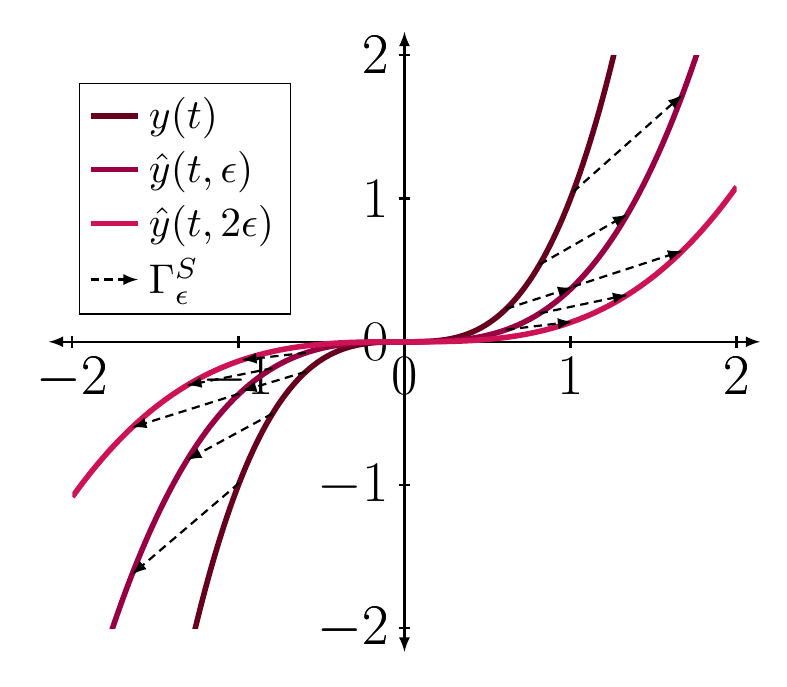
\begin{tikzpicture}
  % The axis of the plot
  \begin{axis}[
    x label style={at={(axis description cs:0.5,-0.15)},anchor=north},
    y label style={at={(axis description cs:-0.15,0.55)},rotate=90,anchor=south,align={center}},    
    legend style={at={(axis description cs:0.01,0.75)},anchor=west,nodes={scale=1.5, transform shape}},
    ymin = -2,
    ymax = 2,
    xmin=-2,
    xmax = 2,
    axis x line*=middle,
    ytick = {-2,-1,...,2},
    xtick = {-2,-1,...,2},
    extra x ticks={0,-2,2},
    extra y ticks = {0,-2,2},
    grid style=dashed,
    label style={font=\huge},
    tick label style={font=\huge},
    legend cell align={left},    
]
\addplot[
color=cube_1,line width=2pt,
]
coordinates {%
(-2.0,-8.0)
(-1.979899497487437,-7.761210029846715)
(-1.9597989949748744,-7.527219694848069)
(-1.9396984924623115,-7.297980267743607)
(-1.9195979899497488,-7.073443021272876)
(-1.899497487437186,-6.853559228175421)
(-1.879396984924623,-6.638280161190792)
(-1.8592964824120604,-6.427557093058536)
(-1.8391959798994975,-6.221341296518196)
(-1.8190954773869348,-6.019584044309323)
(-1.7989949748743719,-5.82223660917146)
(-1.778894472361809,-5.629250263844156)
(-1.7587939698492463,-5.44057628106696)
(-1.7386934673366834,-5.256165933579414)
(-1.7185929648241207,-5.07597049412107)
(-1.6984924623115578,-4.899941235431469)
(-1.678391959798995,-4.728029430250162)
(-1.6582914572864322,-4.5601863513166965)
(-1.6381909547738693,-4.396363271370615)
(-1.6180904522613067,-4.236511463151469)
(-1.5979899497487438,-4.080582199398802)
(-1.5778894472361809,-3.928526752852162)
(-1.557788944723618,-3.7802963962510963)
(-1.5376884422110553,-3.6358424023351525)
(-1.5175879396984926,-3.4951160438438764)
(-1.4974874371859297,-3.358068593516813)
(-1.4773869346733668,-3.224651324093511)
(-1.457286432160804,-3.094815508313517)
(-1.4371859296482412,-2.9685124189163794)
(-1.4170854271356785,-2.8456933286416435)
(-1.3969849246231156,-2.726309510228855)
(-1.3768844221105527,-2.6103122364175615)
(-1.3567839195979898,-2.4976527799473103)
(-1.3366834170854272,-2.3882824135576497)
(-1.3165829145728645,-2.2821524099881247)
(-1.2964824120603016,-2.1792140419782813)
(-1.2763819095477387,-2.0794185822676674)
(-1.2562814070351758,-1.98271730359583)
(-1.236180904522613,-1.889061478702317)
(-1.2160804020100502,-1.7984023803266729)
(-1.1959798994974875,-1.7106912812084465)
(-1.1758793969849246,-1.6258794540871828)
(-1.1557788944723617,-1.5439181717024297)
(-1.135678391959799,-1.4647587067937349)
(-1.1155778894472361,-1.3883523321006435)
(-1.0954773869346734,-1.3146503203627036)
(-1.0753768844221105,-1.2436039443194609)
(-1.0552763819095476,-1.175164476710463)
(-1.035175879396985,-1.1092831902752571)
(-1.015075376884422,-1.045911357753389)
(-0.9949748743718594,-0.9850002518844065)
(-0.9748743718592965,-0.9265011454078554)
(-0.9547738693467336,-0.8703653110632832)
(-0.9346733668341709,-0.8165440215902371)
(-0.914572864321608,-0.7649885497282629)
(-0.8944723618090451,-0.7156501682169081)
(-0.8743718592964824,-0.6684801497957199)
(-0.8542713567839195,-0.623429767204244)
(-0.8341708542713568,-0.5804502931820286)
(-0.8140703517587939,-0.5394930004686191)
(-0.793969849246231,-0.5005091618035632)
(-0.7738693467336684,-0.4634500499264079)
(-0.7537688442211055,-0.4282669375766993)
(-0.7336683417085428,-0.394911097493985)
(-0.7135678391959799,-0.3633338024178111)
(-0.693467336683417,-0.3334863250877248)
(-0.6733668341708543,-0.3053199382432732)
(-0.6532663316582914,-0.2787859146240025)
(-0.6331658291457287,-0.25383552696946016)
(-0.6130653266331658,-0.23042004801919244)
(-0.5929648241206029,-0.20849075051274646)
(-0.5728643216080402,-0.18799890718966925)
(-0.5527638190954773,-0.1688957907895072)
(-0.5326633165829147,-0.15113267405180755)
(-0.5125628140703518,-0.13466082971611676)
(-0.49246231155778886,-0.11943153052198183)
(-0.4723618090452262,-0.10539604920894975)
(-0.4522613065326633,-0.09250565851656706)
(-0.4321608040201004,-0.08071163118438071)
(-0.4120603015075377,-0.06996523995193767)
(-0.3919597989949748,-0.060217757558784515)
(-0.3718592964824121,-0.0514204567444683)
(-0.3517587939698492,-0.04352461024853566)
(-0.3316582914572863,-0.03648149081053353)
(-0.31155778894472363,-0.030242371170008782)
(-0.29145728643216073,-0.024758524066508126)
(-0.27135678391959805,-0.019981222239578503)
(-0.25125628140703515,-0.01586173842876664)
(-0.23115577889447225,-0.012351345373619425)
(-0.21105527638190957,-0.00940131581368371)
(-0.19095477386934667,-0.0069629224885062605)
(-0.170854271356784,-0.00498743813763396)
(-0.1507537688442211,-0.0034261355006135947)
(-0.1306532663316582,-0.0022302873169920156)
(-0.11055276381909551,-0.0013511663263160592)
(-0.09045226130653261,-0.0007400452681325353)
(-0.07035175879396993,-0.00034819688198828666)
(-0.05025125628140703,-0.00012689390743013314)
(-0.03015075376884413,-2.7409084004908513e-05)
(-0.01005025125628145,-1.0151512594410786e-06)
(0.010050251256281229,1.0151512594410112e-06)
(0.03015075376884413,2.7409084004908513e-05)
(0.05025125628140703,0.00012689390743013314)
(0.07035175879396993,0.00034819688198828666)
(0.09045226130653283,0.0007400452681325407)
(0.11055276381909529,0.001351166326316051)
(0.1306532663316582,0.0022302873169920156)
(0.1507537688442211,0.0034261355006135947)
(0.170854271356784,0.00498743813763396)
(0.1909547738693469,0.006962922488506285)
(0.2110552763819098,0.009401315813683739)
(0.23115577889447225,0.012351345373619425)
(0.25125628140703515,0.01586173842876664)
(0.27135678391959805,0.019981222239578503)
(0.29145728643216096,0.02475852406650818)
(0.31155778894472386,0.030242371170008848)
(0.3316582914572863,0.03648149081053353)
(0.3517587939698492,0.04352461024853566)
(0.3718592964824121,0.0514204567444683)
(0.391959798994975,0.06021775755878462)
(0.4120603015075379,0.06996523995193778)
(0.4321608040201004,0.08071163118438071)
(0.4522613065326633,0.09250565851656706)
(0.4723618090452262,0.10539604920894975)
(0.4924623115577891,0.119431530521982)
(0.512562814070352,0.13466082971611693)
(0.5326633165829144,0.15113267405180736)
(0.5527638190954773,0.1688957907895072)
(0.5728643216080402,0.18799890718966925)
(0.5929648241206031,0.20849075051274668)
(0.613065326633166,0.2304200480191927)
(0.6331658291457285,0.2538355269694599)
(0.6532663316582914,0.2787859146240025)
(0.6733668341708543,0.3053199382432732)
(0.6934673366834172,0.3334863250877251)
(0.7135678391959801,0.36333380241781144)
(0.7336683417085426,0.3949110974939847)
(0.7537688442211055,0.4282669375766993)
(0.7738693467336684,0.4634500499264079)
(0.7939698492462313,0.5005091618035636)
(0.8140703517587942,0.5394930004686196)
(0.8341708542713566,0.5804502931820281)
(0.8542713567839195,0.623429767204244)
(0.8743718592964824,0.6684801497957199)
(0.8944723618090453,0.7156501682169086)
(0.9145728643216082,0.7649885497282635)
(0.9346733668341707,0.8165440215902365)
(0.9547738693467336,0.8703653110632832)
(0.9748743718592965,0.9265011454078554)
(0.9949748743718594,0.9850002518844065)
(1.0150753768844223,1.0459113577533896)
(1.0351758793969852,1.1092831902752578)
(1.0552763819095476,1.175164476710463)
(1.0753768844221105,1.2436039443194609)
(1.0954773869346734,1.3146503203627036)
(1.1155778894472363,1.3883523321006443)
(1.1356783919597992,1.4647587067937358)
(1.1557788944723617,1.5439181717024297)
(1.1758793969849246,1.6258794540871828)
(1.1959798994974875,1.7106912812084465)
(1.2160804020100504,1.7984023803266738)
(1.2361809045226133,1.889061478702318)
(1.2562814070351758,1.98271730359583)
(1.2763819095477387,2.0794185822676674)
(1.2964824120603016,2.1792140419782813)
(1.3165829145728645,2.2821524099881247)
(1.3366834170854274,2.388282413557651)
(1.3567839195979898,2.4976527799473103)
(1.3768844221105527,2.6103122364175615)
(1.3969849246231156,2.726309510228855)
(1.4170854271356785,2.8456933286416435)
(1.4371859296482414,2.9685124189163807)
(1.457286432160804,3.094815508313517)
(1.4773869346733668,3.224651324093511)
(1.4974874371859297,3.358068593516813)
(1.5175879396984926,3.4951160438438764)
(1.5376884422110555,3.635842402335154)
(1.557788944723618,3.7802963962510963)
(1.5778894472361809,3.928526752852162)
(1.5979899497487438,4.080582199398802)
(1.6180904522613067,4.236511463151469)
(1.6381909547738696,4.396363271370617)
(1.658291457286432,4.560186351316695)
(1.678391959798995,4.728029430250162)
(1.6984924623115578,4.899941235431469)
(1.7185929648241207,5.07597049412107)
(1.7386934673366836,5.256165933579417)
(1.758793969849246,5.440576281066958)
(1.778894472361809,5.629250263844156)
(1.7989949748743719,5.82223660917146)
(1.8190954773869348,6.019584044309323)
(1.8391959798994977,6.221341296518198)
(1.8592964824120601,6.4275570930585335)
(1.879396984924623,6.638280161190792)
(1.899497487437186,6.853559228175421)
(1.9195979899497488,7.073443021272876)
(1.9396984924623117,7.2979802677436085)
(1.9597989949748746,7.527219694848072)
(1.979899497487437,7.761210029846715)
(2.0,8.0)
};
\addlegendentry{$y(t)$}
\addplot[
color=cube_2,line width=2pt,
]
coordinates {%
(-2.0,-2.9430355293715387)
(-1.979899497487437,-2.855189608594203)
(-1.9597989949748744,-2.7691093749153826)
(-1.9396984924623115,-2.684776902577731)
(-1.9195979899497488,-2.6021742658239044)
(-1.899497487437186,-2.5212835388965558)
(-1.879396984924623,-2.442086796038341)
(-1.8592964824120604,-2.3645661114919148)
(-1.8391959798994975,-2.2887035594999303)
(-1.8190954773869348,-2.2144812143050445)
(-1.7989949748743719,-2.14188115014991)
(-1.778894472361809,-2.0708854412771824)
(-1.7587939698492463,-2.001476161929517)
(-1.7386934673366834,-1.9336353863495672)
(-1.7185929648241207,-1.8673451887799892)
(-1.6984924623115578,-1.8025876434634356)
(-1.678391959798995,-1.7393448246425625)
(-1.6582914572864322,-1.677598806560025)
(-1.6381909547738693,-1.6173316634584758)
(-1.6180904522613067,-1.5585254695805721)
(-1.5979899497487438,-1.5011622991689664)
(-1.5778894472361809,-1.4452242264663144)
(-1.557788944723618,-1.3906933257152707)
(-1.5376884422110553,-1.3375516711584903)
(-1.5175879396984926,-1.2857813370386275)
(-1.4974874371859297,-1.2353643975983364)
(-1.4773869346733668,-1.1862829270802724)
(-1.457286432160804,-1.13851899972709)
(-1.4371859296482412,-1.0920546897814443)
(-1.4170854271356785,-1.0468720714859894)
(-1.3969849246231156,-1.0029532190833799)
(-1.3768844221105527,-0.9602802068162704)
(-1.3567839195979898,-0.9188351089273159)
(-1.3366834170854272,-0.8785999996591717)
(-1.3165829145728645,-0.8395569532544916)
(-1.2964824120603016,-0.8016880439559302)
(-1.2763819095477387,-0.7649753460061424)
(-1.2562814070351758,-0.7294009336477829)
(-1.236180904522613,-0.6949468811235069)
(-1.2160804020100502,-0.6615952626759681)
(-1.1959798994974875,-0.629328152547822)
(-1.1758793969849246,-0.5981276249817226)
(-1.1557788944723617,-0.5679757542203248)
(-1.135678391959799,-0.5388546145062837)
(-1.1155778894472361,-0.5107462800822534)
(-1.0954773869346734,-0.483632825190889)
(-1.0753768844221105,-0.45749632407484475)
(-1.0552763819095476,-0.4323188509767756)
(-1.035175879396985,-0.40808248013933635)
(-1.015075376884422,-0.3847692858051812)
(-0.9949748743718594,-0.3623613422169654)
(-0.9748743718592965,-0.3408407236173431)
(-0.9547738693467336,-0.3201895042489692)
(-0.9346733668341709,-0.30038975835449855)
(-0.914572864321608,-0.2814235601765855)
(-0.8944723618090451,-0.26327298395788484)
(-0.8743718592964824,-0.2459201039410515)
(-0.8542713567839195,-0.22934699436873968)
(-0.8341708542713568,-0.21353572948360452)
(-0.8140703517587939,-0.1984683835283003)
(-0.793969849246231,-0.18412703074548184)
(-0.7738693467336684,-0.17049374537780398)
(-0.7537688442211055,-0.15755060166792112)
(-0.7336683417085428,-0.1452796738584882)
(-0.7135678391959799,-0.13366303619215958)
(-0.693467336683417,-0.12268276291159015)
(-0.6733668341708543,-0.11232092825943463)
(-0.6532663316582914,-0.10255960647834747)
(-0.6331658291457287,-0.09338087181098358)
(-0.6130653266331658,-0.08476679849999742)
(-0.5929648241206029,-0.07669946078804377)
(-0.5728643216080402,-0.06916093291777738)
(-0.5527638190954773,-0.062133289131852745)
(-0.5326633165829147,-0.055598603672924705)
(-0.5125628140703518,-0.04953895078364779)
(-0.49246231155778886,-0.043936404706676736)
(-0.4723618090452262,-0.03877303968466627)
(-0.4522613065326633,-0.03403092996027096)
(-0.4321608040201004,-0.029692149776145534)
(-0.4120603015075377,-0.0257387733749447)
(-0.3919597989949748,-0.022152874999323044)
(-0.3718592964824121,-0.018916528891935323)
(-0.3517587939698492,-0.016011809295436132)
(-0.3316582914572863,-0.013420790452480184)
(-0.31155778894472363,-0.011125546605722169)
(-0.29145728643216073,-0.009108151997816715)
(-0.27135678391959805,-0.007350680871418535)
(-0.25125628140703515,-0.005835207469182264)
(-0.23115577889447225,-0.0045438060337625935)
(-0.21105527638190957,-0.0034585508078142065)
(-0.19095477386934667,-0.002561516033991752)
(-0.170854271356784,-0.0018347759549499204)
(-0.1507537688442211,-0.0012604048133433691)
(-0.1306532663316582,-0.0008204768518267782)
(-0.11055276381909551,-0.0004970663130548226)
(-0.09045226130653261,-0.0002722474396821673)
(-0.07035175879396993,-0.00012809447436348955)
(-0.05025125628140703,-4.668165975345811e-05)
(-0.03015075376884413,-1.0083238506746862e-05)
(-0.01005025125628145,-3.7345327802766984e-07)
(0.010050251256281229,3.7345327802764507e-07)
(0.03015075376884413,1.0083238506746862e-05)
(0.05025125628140703,4.668165975345811e-05)
(0.07035175879396993,0.00012809447436348955)
(0.09045226130653283,0.0002722474396821693)
(0.11055276381909529,0.0004970663130548196)
(0.1306532663316582,0.0008204768518267782)
(0.1507537688442211,0.0012604048133433691)
(0.170854271356784,0.0018347759549499204)
(0.1909547738693469,0.0025615160339917606)
(0.2110552763819098,0.0034585508078142173)
(0.23115577889447225,0.0045438060337625935)
(0.25125628140703515,0.005835207469182264)
(0.27135678391959805,0.007350680871418535)
(0.29145728643216096,0.009108151997816736)
(0.31155778894472386,0.011125546605722193)
(0.3316582914572863,0.013420790452480184)
(0.3517587939698492,0.016011809295436132)
(0.3718592964824121,0.018916528891935323)
(0.391959798994975,0.022152874999323082)
(0.4120603015075379,0.02573877337494474)
(0.4321608040201004,0.029692149776145534)
(0.4522613065326633,0.03403092996027096)
(0.4723618090452262,0.03877303968466627)
(0.4924623115577891,0.04393640470667679)
(0.512562814070352,0.04953895078364785)
(0.5326633165829144,0.055598603672924636)
(0.5527638190954773,0.062133289131852745)
(0.5728643216080402,0.06916093291777738)
(0.5929648241206031,0.07669946078804385)
(0.613065326633166,0.08476679849999752)
(0.6331658291457285,0.09338087181098348)
(0.6532663316582914,0.10255960647834747)
(0.6733668341708543,0.11232092825943463)
(0.6934673366834172,0.12268276291159025)
(0.7135678391959801,0.13366303619215972)
(0.7336683417085426,0.14527967385848806)
(0.7537688442211055,0.15755060166792112)
(0.7738693467336684,0.17049374537780398)
(0.7939698492462313,0.184127030745482)
(0.8140703517587942,0.19846838352830046)
(0.8341708542713566,0.21353572948360436)
(0.8542713567839195,0.22934699436873968)
(0.8743718592964824,0.2459201039410515)
(0.8944723618090453,0.26327298395788507)
(0.9145728643216082,0.2814235601765857)
(0.9346733668341707,0.3003897583544984)
(0.9547738693467336,0.3201895042489692)
(0.9748743718592965,0.3408407236173431)
(0.9949748743718594,0.3623613422169654)
(1.0150753768844223,0.3847692858051815)
(1.0351758793969852,0.40808248013933657)
(1.0552763819095476,0.4323188509767756)
(1.0753768844221105,0.45749632407484475)
(1.0954773869346734,0.483632825190889)
(1.1155778894472363,0.5107462800822538)
(1.1356783919597992,0.538854614506284)
(1.1557788944723617,0.5679757542203248)
(1.1758793969849246,0.5981276249817226)
(1.1959798994974875,0.629328152547822)
(1.2160804020100504,0.6615952626759685)
(1.2361809045226133,0.6949468811235073)
(1.2562814070351758,0.7294009336477829)
(1.2763819095477387,0.7649753460061424)
(1.2964824120603016,0.8016880439559302)
(1.3165829145728645,0.8395569532544916)
(1.3366834170854274,0.8785999996591722)
(1.3567839195979898,0.9188351089273159)
(1.3768844221105527,0.9602802068162704)
(1.3969849246231156,1.0029532190833799)
(1.4170854271356785,1.0468720714859894)
(1.4371859296482414,1.0920546897814447)
(1.457286432160804,1.13851899972709)
(1.4773869346733668,1.1862829270802724)
(1.4974874371859297,1.2353643975983364)
(1.5175879396984926,1.2857813370386275)
(1.5376884422110555,1.3375516711584907)
(1.557788944723618,1.3906933257152707)
(1.5778894472361809,1.4452242264663144)
(1.5979899497487438,1.5011622991689664)
(1.6180904522613067,1.5585254695805721)
(1.6381909547738696,1.6173316634584765)
(1.658291457286432,1.6775988065600242)
(1.678391959798995,1.7393448246425625)
(1.6984924623115578,1.8025876434634356)
(1.7185929648241207,1.8673451887799892)
(1.7386934673366836,1.9336353863495683)
(1.758793969849246,2.0014761619295167)
(1.778894472361809,2.0708854412771824)
(1.7989949748743719,2.14188115014991)
(1.8190954773869348,2.2144812143050445)
(1.8391959798994977,2.288703559499931)
(1.8592964824120601,2.364566111491914)
(1.879396984924623,2.442086796038341)
(1.899497487437186,2.5212835388965558)
(1.9195979899497488,2.6021742658239044)
(1.9396984924623117,2.684776902577732)
(1.9597989949748746,2.7691093749153834)
(1.979899497487437,2.855189608594203)
(2.0,2.9430355293715387)
};
\addlegendentry{$\hat{y}(t,\epsilon)$}
\addplot[
color=cube_3,line width=2pt,
]
coordinates {%
(-2.0,-1.0826822658929016)
(-1.979899497487437,-1.0503655576481445)
(-1.9597989949748744,-1.0186984093864728)
(-1.9396984924623115,-0.9876742265902916)
(-1.9195979899497488,-0.9572864147420062)
(-1.899497487437186,-0.9275283793240214)
(-1.879396984924623,-0.8983935258187429)
(-1.8592964824120604,-0.8698752597085759)
(-1.8391959798994975,-0.8419669864759253)
(-1.8190954773869348,-0.8146621116031969)
(-1.7989949748743719,-0.7879540405727951)
(-1.778894472361809,-0.7618361788671256)
(-1.7587939698492463,-0.7363019319685941)
(-1.7386934673366834,-0.7113447053596048)
(-1.7185929648241207,-0.686957904522564)
(-1.6984924623115578,-0.6631349349398759)
(-1.678391959798995,-0.6398692020939463)
(-1.6582914572864322,-0.6171541114671806)
(-1.6381909547738693,-0.5949830685419834)
(-1.6180904522613067,-0.5733494788007606)
(-1.5979899497487438,-0.5522467477259169)
(-1.5778894472361809,-0.5316682807998577)
(-1.557788944723618,-0.5116074835049884)
(-1.5376884422110553,-0.4920577613237142)
(-1.5175879396984926,-0.4730125197384403)
(-1.4974874371859297,-0.4544651642315715)
(-1.4773869346733668,-0.4364091002855135)
(-1.457286432160804,-0.4188377333826714)
(-1.4371859296482412,-0.4017444690054505)
(-1.4170854271356785,-0.385122712636256)
(-1.3969849246231156,-0.3689658697574929)
(-1.3768844221105527,-0.3532673458515666)
(-1.3567839195979898,-0.33802054640088236)
(-1.3366834170854272,-0.3232188768878455)
(-1.3165829145728645,-0.3088557427948611)
(-1.2964824120603016,-0.2949245496043343)
(-1.2763819095477387,-0.2814187027986704)
(-1.2562814070351758,-0.26833160786027466)
(-1.236180904522613,-0.2556566702715525)
(-1.2160804020100502,-0.24338729551490876)
(-1.1959798994974875,-0.23151688907274898)
(-1.1758793969849246,-0.2200388564274781)
(-1.1557788944723617,-0.20894660306150156)
(-1.135678391959799,-0.19823353445722464)
(-1.1155778894472361,-0.18789305609705237)
(-1.0954773869346734,-0.17791857346339013)
(-1.0753768844221105,-0.16830349203864298)
(-1.0552763819095476,-0.15904121730521625)
(-1.035175879396985,-0.15012515474551527)
(-1.015075376884422,-0.14154870984194506)
(-0.9949748743718594,-0.13330528807691103)
(-0.9748743718592965,-0.1253882949328182)
(-0.9547738693467336,-0.11779113589207195)
(-0.9346733668341709,-0.11050721643707753)
(-0.914572864321608,-0.10352994205024005)
(-0.8944723618090451,-0.09685271821396478)
(-0.8743718592964824,-0.09046895041065704)
(-0.8542713567839195,-0.08437204412272188)
(-0.8341708542713568,-0.07855540483256472)
(-0.8140703517587939,-0.0730124380225906)
(-0.793969849246231,-0.06773654917520484)
(-0.7738693467336684,-0.06272114377281271)
(-0.7537688442211055,-0.05795962729781933)
(-0.7336683417085428,-0.053445405232630035)
(-0.7135678391959799,-0.049171883059649944)
(-0.693467336683417,-0.04513246626128434)
(-0.6733668341708543,-0.04132056031993848)
(-0.6532663316582914,-0.037729570718017504)
(-0.6331658291457287,-0.034352902937926734)
(-0.6130653266331658,-0.031183962462071307)
(-0.5929648241206029,-0.028216154772856498)
(-0.5728643216080402,-0.02544288535268755)
(-0.5527638190954773,-0.02285755968396964)
(-0.5326633165829147,-0.02045358324910804)
(-0.5125628140703518,-0.018224361530507934)
(-0.49246231155778886,-0.016163300010574564)
(-0.4723618090452262,-0.014263804171713185)
(-0.4522613065326633,-0.012519279496328977)
(-0.4321608040201004,-0.010923131466827185)
(-0.4120603015075377,-0.009468765565613055)
(-0.3919597989949748,-0.008149587275091777)
(-0.3718592964824121,-0.00695900207766861)
(-0.3517587939698492,-0.00589041545574875)
(-0.3316582914572863,-0.004937232891737439)
(-0.31155778894472363,-0.004092859868039909)
(-0.29145728643216073,-0.0033507018670613695)
(-0.27135678391959805,-0.0027041643712070614)
(-0.25125628140703515,-0.0021466528628821973)
(-0.23115577889447225,-0.0016715728244920108)
(-0.21105527638190957,-0.0012723297384417307)
(-0.19095477386934667,-0.0009423290871365749)
(-0.170854271356784,-0.0006749763529817762)
(-0.1507537688442211,-0.0004636770183825547)
(-0.1306532663316582,-0.00030183656574413946)
(-0.11055276381909551,-0.00018286047747175733)
(-0.09045226130653261,-0.00010015423597063166)
(-0.07035175879396993,-4.7123323645990185e-05)
(-0.05025125628140703,-1.717322290305758e-05)
(-0.03015075376884413,-3.7094161470604043e-06)
(-0.01005025125628145,-1.3738578322446248e-07)
(0.010050251256281229,1.3738578322445337e-07)
(0.03015075376884413,3.7094161470604043e-06)
(0.05025125628140703,1.717322290305758e-05)
(0.07035175879396993,4.7123323645990185e-05)
(0.09045226130653283,0.00010015423597063239)
(0.11055276381909529,0.00018286047747175622)
(0.1306532663316582,0.00030183656574413946)
(0.1507537688442211,0.0004636770183825547)
(0.170854271356784,0.0006749763529817762)
(0.1909547738693469,0.0009423290871365782)
(0.2110552763819098,0.0012723297384417348)
(0.23115577889447225,0.0016715728244920108)
(0.25125628140703515,0.0021466528628821973)
(0.27135678391959805,0.0027041643712070614)
(0.29145728643216096,0.003350701867061377)
(0.31155778894472386,0.004092859868039918)
(0.3316582914572863,0.004937232891737439)
(0.3517587939698492,0.00589041545574875)
(0.3718592964824121,0.00695900207766861)
(0.391959798994975,0.008149587275091791)
(0.4120603015075379,0.00946876556561307)
(0.4321608040201004,0.010923131466827185)
(0.4522613065326633,0.012519279496328977)
(0.4723618090452262,0.014263804171713185)
(0.4924623115577891,0.01616330001057459)
(0.512562814070352,0.018224361530507955)
(0.5326633165829144,0.020453583249108016)
(0.5527638190954773,0.02285755968396964)
(0.5728643216080402,0.02544288535268755)
(0.5929648241206031,0.028216154772856526)
(0.613065326633166,0.031183962462071342)
(0.6331658291457285,0.03435290293792669)
(0.6532663316582914,0.037729570718017504)
(0.6733668341708543,0.04132056031993848)
(0.6934673366834172,0.04513246626128437)
(0.7135678391959801,0.049171883059649986)
(0.7336683417085426,0.053445405232629986)
(0.7537688442211055,0.05795962729781933)
(0.7738693467336684,0.06272114377281271)
(0.7939698492462313,0.0677365491752049)
(0.8140703517587942,0.07301243802259066)
(0.8341708542713566,0.07855540483256467)
(0.8542713567839195,0.08437204412272188)
(0.8743718592964824,0.09046895041065704)
(0.8944723618090453,0.09685271821396485)
(0.9145728643216082,0.10352994205024012)
(0.9346733668341707,0.11050721643707746)
(0.9547738693467336,0.11779113589207195)
(0.9748743718592965,0.1253882949328182)
(0.9949748743718594,0.13330528807691103)
(1.0150753768844223,0.14154870984194515)
(1.0351758793969852,0.15012515474551535)
(1.0552763819095476,0.15904121730521625)
(1.0753768844221105,0.16830349203864298)
(1.0954773869346734,0.17791857346339013)
(1.1155778894472363,0.18789305609705248)
(1.1356783919597992,0.19823353445722477)
(1.1557788944723617,0.20894660306150156)
(1.1758793969849246,0.2200388564274781)
(1.1959798994974875,0.23151688907274898)
(1.2160804020100504,0.24338729551490887)
(1.2361809045226133,0.25565667027155264)
(1.2562814070351758,0.26833160786027466)
(1.2763819095477387,0.2814187027986704)
(1.2964824120603016,0.2949245496043343)
(1.3165829145728645,0.3088557427948611)
(1.3366834170854274,0.3232188768878457)
(1.3567839195979898,0.33802054640088236)
(1.3768844221105527,0.3532673458515666)
(1.3969849246231156,0.3689658697574929)
(1.4170854271356785,0.385122712636256)
(1.4371859296482414,0.4017444690054507)
(1.457286432160804,0.4188377333826714)
(1.4773869346733668,0.4364091002855135)
(1.4974874371859297,0.4544651642315715)
(1.5175879396984926,0.4730125197384403)
(1.5376884422110555,0.4920577613237144)
(1.557788944723618,0.5116074835049884)
(1.5778894472361809,0.5316682807998577)
(1.5979899497487438,0.5522467477259169)
(1.6180904522613067,0.5733494788007606)
(1.6381909547738696,0.5949830685419836)
(1.658291457286432,0.6171541114671804)
(1.678391959798995,0.6398692020939463)
(1.6984924623115578,0.6631349349398759)
(1.7185929648241207,0.686957904522564)
(1.7386934673366836,0.7113447053596051)
(1.758793969849246,0.7363019319685938)
(1.778894472361809,0.7618361788671256)
(1.7989949748743719,0.7879540405727951)
(1.8190954773869348,0.8146621116031969)
(1.8391959798994977,0.8419669864759256)
(1.8592964824120601,0.8698752597085756)
(1.879396984924623,0.8983935258187429)
(1.899497487437186,0.9275283793240214)
(1.9195979899497488,0.9572864147420062)
(1.9396984924623117,0.9876742265902919)
(1.9597989949748746,1.0186984093864733)
(1.979899497487437,1.0503655576481445)
(2.0,1.0826822658929016)
};
\addlegendentry{$\hat{y}(t,2\epsilon)$}
\addplot[
color=black,->,>=latex,densely dashed
]
coordinates {%
(-0.9949748743718594,-0.9850002518844065)
(-1.001720440990133,-0.9916781942015903)
(-1.0085117400888677,-0.9984014105311476)
(-1.015349081717595,-1.0051702078143632)
(-1.0222327780278688,-1.0119848950734724)
(-1.0291631432875172,-1.018845783425768)
(-1.0361404938949894,-1.0257531860978049)
(-1.0431651483937994,-1.0327074184396992)
(-1.050237427487072,-1.0397087979395263)
(-1.057357654052181,-1.0467576442378148)
(-1.0645261531554906,-1.0538542791421395)
(-1.0717432520671974,-1.0609990266418126)
(-1.07900928027627,-1.0681922129226762)
(-1.0863245695054922,-1.0754341663819935)
(-1.0936894537266066,-1.0827252176434405)
(-1.101104269175563,-1.0900656995722022)
(-1.1085693543678683,-1.0974559472901675)
(-1.1160850501140407,-1.104896298191229)
(-1.1236516995351693,-1.1123870919566876)
(-1.1312696480785795,-1.1199286705707594)
(-1.138939243533603,-1.127521378336188)
(-1.1466608360474562,-1.1351655618899645)
(-1.1544347781412267,-1.1428615702191525)
(-1.1622614247259657,-1.1506097546768204)
(-1.1701411331188916,-1.1584104689980819)
(-1.178074263059704,-1.1662640693162458)
(-1.1860611767270062,-1.1741709141790753)
(-1.1941022387548397,-1.182131364565156)
(-1.202197816249332,-1.190145783900377)
(-1.2103482788054571,-1.1982145380745222)
(-1.2185539985239067,-1.2063379954579745)
(-1.2268153500280798,-1.2145165269185336)
(-1.2351327104811862,-1.2227505058383483)
(-1.2435064596034637,-1.2310403081309613)
(-1.2519369796895152,-1.2393863122584725)
(-1.2604246556257617,-1.2477888992488162)
(-1.2689698749080132,-1.2562484527131577)
(-1.27757302765916,-1.2647653588634054)
(-1.2862345066469838,-1.2733400065298441)
(-1.2949547073020875,-1.2819727871788855)
(-1.3037340277359506,-1.2906640949309416)
(-1.312572868759102,-1.2994143265784157)
(-1.3214716338994204,-1.3082238816038203)
(-1.3304307294205557,-1.3170931621980122)
(-1.3394505643404782,-1.3260225732785564)
(-1.3485315504501494,-1.3350125225082112)
(-1.3576741023323244,-1.344063420313539)
(-1.3668786373804775,-1.3531756799036452)
(-1.3761455758178585,-1.3623497172890415)
(-1.3854753407166778,-1.37158595130064)
(-1.3948683580174208,-1.380884803608873)
(-1.4043250565482943,-1.3902466987429445)
(-1.4138458680448034,-1.3996720641102116)
(-1.4234312271694627,-1.4091613300156973)
(-1.43308157153164,-1.4187149296817358)
(-1.4427973417075346,-1.4283332992677509)
(-1.4525789812602927,-1.4380168778901676)
(-1.4624269367602554,-1.4477661076424602)
(-1.4723416578053492,-1.4575814336153359)
(-1.482323597041609,-1.4674633039170542)
(-1.492373210183846,-1.4774121696938844)
(-1.502490956036451,-1.487428485150704)
(-1.512677296514341,-1.4975127075717338)
(-1.522932696664047,-1.5076652973414135)
(-1.533257624684948,-1.517886717965423)
(-1.5436525519506417,-1.5281774360918403)
(-1.5541179530304676,-1.538537921532448)
(-1.5646543057111726,-1.5489686472841804)
(-1.5752620910187225,-1.5594700895507188)
(-1.5859417932402646,-1.570042727764232)
(-1.596693899946236,-1.5806870446072634)
(-1.6075189020126226,-1.5914035260347685)
(-1.6184172936433718,-1.6021926612962996)
(-1.6293895723929528,-1.6130549429583427)
(-1.6404362391890723,-1.623990866926805)
};
\addlegendentry{$\Gamma_{\epsilon}^{S}$}
\addplot[
forget plot,
color=black,->,>=latex,densely dashed
]
coordinates {%
(-0.793969849246231,-0.5005091618035632)
(-0.7993526751335402,-0.5039024313030906)
(-0.804771994616369,-0.5073187059317449)
(-0.8102280551079796,-0.5107581416559076)
(-0.8157211056990064,-0.5142208954993558)
(-0.8212513971688268,-0.5177071255504302)
(-0.8268191819970114,-0.521216990969253)
(-0.8324247143748499,-0.5247506519949937)
(-0.8380682502169564,-0.5283082699531854)
(-0.8437500471729522,-0.5318900072630887)
(-0.8494703646392296,-0.535496027445108)
(-0.8552294637707937,-0.5391264951282566)
(-0.861027607493185,-0.5427815760576719)
(-0.8668650605144834,-0.5464614371021832)
(-0.872742089337393,-0.5501662462619294)
(-0.8786589622714086,-0.5538961726760294)
(-0.8846159494450665,-0.5576513866303031)
(-0.8906133228182747,-0.5614320595650464)
(-0.8966513561947309,-0.5652383640828579)
(-0.9027303252344219,-0.5690704739565188)
(-0.9088505074662082,-0.5729285641369262)
(-0.9150121823004952,-0.5768128107610806)
(-0.9212156310419888,-0.5807233911601273)
(-0.9274611369025381,-0.5846604838674516)
(-0.9337489850140648,-0.5886242686268304)
(-0.9400794624415819,-0.5926149264006374)
(-0.9464528581962977,-0.5966326393781058)
(-0.9528694632488113,-0.6006775909836448)
(-0.9593295705423962,-0.6047499658852142)
(-0.9658334750063746,-0.6088499500027557)
(-0.9723814735695818,-0.6129777305166797)
(-0.978973865173922,-0.6171334958764119)
(-0.9856109507880171,-0.621317435808996)
(-0.9922930334209457,-0.6255297413277563)
(-0.9990204181360777,-0.6297706047410175)
(-1.0057934120650016,-0.6340402196608846)
(-1.0126123244215457,-0.638338781012082)
(-1.019477466515895,-0.6426664850408524)
(-1.0263891517688049,-0.647023529323917)
(-1.033347695725908,-0.6514101127774945)
(-1.040353416072122,-0.6558264356663833)
(-1.0474066326461517,-0.6602726996131039)
(-1.0545076674550928,-0.664749107607104)
(-1.0616568446891301,-0.6692558640140258)
(-1.0688544907363409,-0.6737931745850358)
(-1.0761009341975938,-0.6783612464662186)
(-1.0833965059015516,-0.6829602882080332)
(-1.0907415389197748,-0.6875905097748352)
(-1.0981363685819272,-0.6922521225544613)
(-1.1055813324910861,-0.6969453393678813)
(-1.1130767705391538,-0.7016703744789128)
(-1.120623024922376,-0.7064274436040047)
(-1.1282204401569642,-0.7112167639220839)
(-1.1358693630948236,-0.7160385540844717)
(-1.1435701429393892,-0.7208930342248656)
(-1.151323131261568,-0.725780425969389)
(-1.159128682015789,-0.7307009524467095)
(-1.1669871515561632,-0.7356548382982261)
(-1.174898898652753,-0.740642309688324)
(-1.1828642845079504,-0.7456635943147009)
(-1.190883672772968,-0.7507189214187612)
(-1.1989574295644403,-0.7558085217960829)
(-1.2070859234811404,-0.7609326278069538)
(-1.215269525620805,-0.7660914733869794)
(-1.2235086095970795,-0.7712852940577632)
(-1.2318035515565724,-0.7765143269376598)
(-1.2401547301960294,-0.7817788107525989)
(-1.2485625267796223,-0.7870789858469858)
(-1.257027325156354,-0.7924150941946722)
(-1.2655495117775846,-0.7977873794100051)
(-1.2741294757146726,-0.8031960867589475)
(-1.282767608676739,-0.8086414631702761)
(-1.291464305028549,-0.8141237572468546)
(-1.3002199618085175,-0.8196432192769835)
(-1.3090349787468352,-0.8252001012458268)
};
\addplot[
forget plot,
color=black,->,>=latex,densely dashed
]
coordinates {%
(-0.5929648241206029,-0.20849075051274646)
(-0.5969849092769478,-0.20990424173056788)
(-0.6010322491438704,-0.21132731590311482)
(-0.6051070284983645,-0.21276003799932386)
(-0.609209433370144,-0.2142024734285973)
(-0.6133396510501364,-0.21565468804378923)
(-0.6174978700990339,-0.21711674814421214)
(-0.6216842803559005,-0.2185887204786636)
(-0.6258990729468408,-0.22007067224847376)
(-0.6301424402937238,-0.22156267111057315)
(-0.6344145761229689,-0.22306478518058173)
(-0.6387156754743902,-0.22457708303591847)
(-0.6430459347101002,-0.22609963371893216)
(-0.647405551523475,-0.22763250674005361)
(-0.6517947249481795,-0.22917577208096887)
(-0.6562136553672545,-0.23072950019781444)
(-0.6606625445222648,-0.23229376202439364)
(-0.6651415955225088,-0.23386862897541505)
(-0.6696510128542926,-0.235454172949753)
(-0.6741910023902644,-0.23705046633372992)
(-0.6787617713988137,-0.23865758200442108)
(-0.6833635285535343,-0.24027559333298174)
(-0.687996483942751,-0.24190457418799685)
(-0.6926608490791106,-0.2435445989388534)
(-0.6973568369092382,-0.24519574245913564)
(-0.7020846618234599,-0.24685808013004348)
(-0.7068445396655894,-0.24853168784383384)
(-0.7116366877427831,-0.2502166420072854)
(-0.7164613248354604,-0.2519130195451869)
(-0.7213186712072924,-0.2536208979038493)
(-0.7262089486152573,-0.25534035505464103)
(-0.7311323803197646,-0.257071469497548)
(-0.7360891910948482,-0.25881432026475754)
(-0.7410796072384277,-0.26056898692426617)
(-0.7461038565826402,-0.2623355495835125)
(-0.7511621685042417,-0.26411408889303445)
(-0.7562547739350783,-0.26590468605015094)
(-0.7613819053726304,-0.2677074228026692)
(-0.7665437968906265,-0.26952238145261687)
(-0.7717406841497287,-0.27134964485999896)
(-0.7769728044082935,-0.2731892964465816)
(-0.782240396533202,-0.2750414201996995)
(-0.7875437010107654,-0.2769061006760914)
(-0.7928829599577047,-0.2787834230057594)
(-0.7982584171322039,-0.28067347289585626)
(-0.8036703179450384,-0.2825763366345979)
(-0.809118909470779,-0.28449210109520273)
(-0.8146044404590722,-0.28642085373985804)
(-0.8201271613459963,-0.28836268262371273)
(-0.8256873242654946,-0.2903176763988976)
(-0.831285183060887,-0.2922859243185724)
(-0.8369209932964581,-0.29426751624100095)
(-0.842595012269125,-0.29626254263365304)
(-0.8483074990201847,-0.2982710945773351)
(-0.8540587143471388,-0.30029326377034815)
(-0.8598489208156013,-0.3023291425326741)
(-0.8656783827712853,-0.304378823810191)
(-0.8715473663520712,-0.3064424011789156)
(-0.8774561395001573,-0.3085199688492762)
(-0.8834049719742921,-0.31061162167041334)
(-0.8893941353620899,-0.31271745513451016)
(-0.8954239030924301,-0.3148375653811518)
(-0.9014945504479402,-0.316972049201715)
(-0.9076063545775632,-0.31912100404378646)
(-0.9137595945092113,-0.3212845280156121)
(-0.9199545511625034,-0.3234627198905758)
(-0.9261915073615916,-0.32565567911170923)
(-0.9324707478480724,-0.3278635057962313)
(-0.938792559293986,-0.3300863007401191)
(-0.945157230314905,-0.3323241654227098)
(-0.95156505148311,-0.3345772020113335)
(-0.9580163153408557,-0.3368455133659774)
(-0.9645113164137264,-0.33912920304398175)
(-0.9710503512240827,-0.34142837530476816)
(-0.9776337183045984,-0.34374313511459875)
};
\addplot[
forget plot,
color=black,->,>=latex,densely dashed
]
coordinates {%
(0.613065326633166,0.2304200480191927)
(0.6172216858626073,0.2319822118729086)
(0.6214062236911206,0.23355496662757622)
(0.6256191311593263,0.23513838408563972)
(0.6298606006030305,0.23673253653633777)
(0.6341308256620057,0.23833749675900356)
(0.638430001288832,0.23995333802638777)
(0.6427583237577958,0.24158013410800333)
(0.6471159906738527,0.24321795927349385)
(0.6515032009816469,0.24486688829602385)
(0.6559201549745953,0.24652699645569265)
(0.660367054304031,0.2481983595429712)
(0.664844101988409,0.24988105386216222)
(0.6693515024225761,0.25157515623488375)
(0.6738894613871012,0.2532807440035762)
(0.6784581860576703,0.2549978950350338)
(0.6830578850145453,0.256726687723959)
(0.6876887682520858,0.2584672009965418)
(0.6923510471883368,0.2602195143140631)
(0.6970449346746805,0.2619837076765221)
(0.7017706450055535,0.2637598616262889)
(0.7065283939282307,0.2655480572517814)
(0.7113183986526752,0.2673483761911675)
(0.7161408778614538,0.26916090063609216)
(0.7209960517197213,0.27098571333542937)
(0.7258841418852724,0.2728228975990607)
(0.7308053715186605,0.274672537301678)
(0.7357599652933863,0.2765347168866132)
(0.7407481494061544,0.27840952136969294)
(0.745770151587201,0.2802970363431203)
(0.7508262011106901,0.28219734797938234)
(0.7559165288051807,0.2841105430351839)
(0.7610413670641655,0.2860367088554089)
(0.7662009498566799,0.2879759333771074)
(0.7713955127379843,0.289928305133511)
(0.776625292860318,0.29189391325807384)
(0.7818905289837255,0.29387284748854264)
(0.7871914614869573,0.2958651981710533)
(0.7925283323784447,0.2978710562642554)
(0.797901385307347,0.2998905133434651)
(0.8033108655746768,0.3019236616048458)
(0.8087570201444974,0.3039705938696171)
(0.8142400976551986,0.30603140358829284)
(0.8197603484308478,0.308106184844947)
(0.825318024492618,0.31019503236150947)
(0.8309133795702943,0.3122980415020901)
(0.8365466691138567,0.31441530827733266)
(0.8422181503051429,0.3165469293487982)
(0.8479280820695898,0.3186930020333775)
(0.8536767250880543,0.32085362430773484)
(0.859464341808714,0.3230288948127802)
(0.8652911964590503,0.3252189128581731)
(0.8711575550579094,0.3274237784268562)
(0.8770636854276489,0.3296435921796201)
(0.8830098572063643,0.33187845545969885)
(0.8889963418601984,0.33412847029739656)
(0.8950234126957362,0.33639373941474576)
(0.9010913448724809,0.3386743662301966)
(0.9072004154154174,0.3409704548633388)
(0.9133509032276584,0.343282110139655)
(0.9195430891031782,0.345609437595306)
(0.9257772557396317,0.3479525434819496)
(0.9320536877512607,0.350311534771591)
(0.9383726716818879,0.35268651916146637)
(0.9447344960179985,0.35507760507896013)
(0.9511394512019108,0.3574849016865546)
(0.9575878296450359,0.3599085188868141)
(0.9640799257412279,0.36234856732740195)
(0.9706160358802233,0.3648051584061325)
(0.9771964584611734,0.36727840427605657)
(0.9838214939062667,0.3697684178505817)
(0.9904914446744445,0.37227531280862713)
(0.9972066152752092,0.3747992035998137)
(1.0039673122825268,0.3773402054496891)
(1.0107738443488226,0.37989843436498794)
};
\addplot[
forget plot,
color=black,->,>=latex,densely dashed
]
coordinates {%
(0.8140703517587942,0.5394930004686196)
(0.8195894517191998,0.5431505661705182)
(0.8251459691636192,0.5468329288333635)
(0.8307401577689414,0.5505402565715034)
(0.8363722729318929,0.5542727186390396)
(0.8420425717806961,0.5580304854375546)
(0.8477513131868095,0.5618137285238919)
(0.8534987577767451,0.5656226206179872)
(0.8592851679439683,0.5694573356107552)
(0.8651108078608754,0.5733180485720266)
(0.870975943490856,0.5772049357585424)
(0.8768808426004344,0.5811181746219998)
(0.8828257747714938,0.5850579438171535)
(0.8888110114135847,0.5890244232099726)
(0.8948368257763146,0.5930177938858516)
(0.9009034929618244,0.5970382381578782)
(0.907011289937347,0.6010859395751559)
(0.9131604955478515,0.6051610829311842)
(0.919351390528775,0.6092638542722958)
(0.925584257518838,0.6133944409061487)
(0.931859381072948,0.6175530314102791)
(0.9381770476751916,0.6217398156407096)
(0.9445375457519128,0.625954984740618)
(0.9509411656848811,0.6301987311490627)
(0.9573881998245478,0.6344712486097686)
(0.9638789425033945,0.6387727321799727)
(0.9704136900493688,0.6431033782393285)
(0.9769927407994144,0.6474633844988724)
(0.9836163951130901,0.651852950010049)
(0.9902849553862831,0.6562722751737994)
(0.9969987260650146,0.6607215617497098)
(1.0037580136593383,0.6652010128652227)
(1.0105631267573343,0.6697108330249109)
(1.0174143760391978,0.6742512281198131)
(1.0243120742914218,0.6788224054368346)
(1.031256536421078,0.68342457366821)
(1.0382480794701927,0.6880579429210311)
(1.045287022630222,0.6927227247268392)
(1.0523736872566232,0.6974191320512824)
(1.0595083968835262,0.7021473793038376)
(1.0666914772385052,0.7069076823476009)
(1.0739232562574472,0.7117002585091401)
(1.081204064099526,0.7165253265884187)
(1.0885342331622732,0.7213831068687838)
(1.095914098096755,0.7262738211270233)
(1.1033439958228497,0.7311976926434909)
(1.1108242655446292,0.7361549462122993)
(1.1183552487658455,0.7411458081515836)
(1.1259372893055206,0.746170506313833)
(1.1335707333136458,0.7512292700962938)
(1.1412559292869808,0.7563223304514416)
(1.1489932280849682,0.7614499198975259)
(1.1567829829457486,0.7666122725291845)
(1.1646255495022877,0.771809624028132)
(1.1725212857986147,0.7770422116739188)
(1.180470552306165,0.782310274354764)
(1.1884737119402398,0.7876140525784617)
(1.1965311300765729,0.7929537884833613)
(1.204643174568013,0.7983297258494217)
(1.2128102157613168,0.803742110109341)
(1.221032626514056,0.8091911883597612)
(1.2293107822116418,0.8146772093725498)
(1.237645060784461,0.8202004236061565)
(1.2460358427251297,0.825761083217048)
(1.2544835111058668,0.83135944207122)
(1.2629884515959797,0.8369957557557867)
(1.2715510524794738,0.8426702815906498)
(1.2801717046727779,0.8483832786402464)
(1.2888508017425913,0.8541350077253752)
(1.297588739923853,0.8599257314351055)
(1.3063859181378294,0.8657557141387645)
(1.3152427380103278,0.8716252219980066)
(1.3241596038900316,0.8775345229789654)
(1.3331369228669616,0.8834838868644872)
(1.3421751047910595,0.8894735852664474)
};
\addplot[
forget plot,
color=black,->,>=latex,densely dashed
]
coordinates {%
(1.0150753768844223,1.0459113577533896)
(1.0219572175757923,1.0530022551441287)
(1.0288857146361177,1.0601412262319678)
(1.0358611843785566,1.0673285969390327)
(1.0428839452607552,1.0745646953970827)
(1.0499543178993864,1.0818498519624904)
(1.057072625084787,1.0891843992313242)
(1.0642391917956946,1.0965686720545322)
(1.071454345214084,1.1040030075532308)
(1.0787184147401039,1.1114877451340928)
(1.0860317320071167,1.119023226504846)
(1.0933946308968379,1.1266097956898713)
(1.1008074475545786,1.134247799045909)
(1.108270520404593,1.1419375852778726)
(1.1157841901655279,1.1496795054547668)
(1.1233487998659786,1.1574739130257166)
(1.1309646948601486,1.1653211638361032)
(1.1386322228436172,1.173221616143809)
(1.1463517338692133,1.1811756306355747)
(1.1541235803629954,1.1891835704434657)
(1.1619481171403425,1.1972458011614493)
(1.1698257014221525,1.2053626908620874)
(1.1777566928511505,1.2135346101133397)
(1.1857414535083084,1.2217619319954809)
(1.1937803479293745,1.2300450321181335)
(1.2018737431215165,1.2383842886374177)
(1.2100220085800772,1.2467800822732125)
(1.2182255163054425,1.2552327963265397)
(1.2264846408200258,1.2637428166970621)
(1.2347997591853654,1.272310531900701)
(1.2431712510193391,1.2809363330873749)
(1.2515994985134957,1.2896206140588546)
(1.2600848864505032,1.298363771286744)
(1.2686278022217157,1.3071662039305803)
(1.2772286358448592,1.3160283138560553)
(1.2858877799818378,1.3249505056533657)
(1.29460562995666,1.3339331866556796)
(1.3033825837734865,1.3429767669577375)
(1.3122190421348017,1.3520816594345715)
(1.3211154084597054,1.3612482797603556)
(1.3300720889023334,1.370477046427384)
(1.339089492370397,1.3797683807651753)
(1.3481680305438533,1.3891227069597083)
(1.3573081178936985,1.3985404520727884)
(1.3665101717008918,1.4080220460615442)
(1.375774612075405,1.417567921798057)
(1.3851018619754019,1.4271785150891219)
(1.3944923472265478,1.436854264696146)
(1.4039464965414516,1.4465956123551782)
(1.4134647415392372,1.4564030027970771)
(1.4230475167652477,1.4662768837678135)
(1.4326952597108862,1.4762177060489134)
(1.4424084108335875,1.4862259234780366)
(1.4521874135769266,1.4963019929696961)
(1.4620327143908651,1.5064463745361198)
(1.4719447627521314,1.5166595313082496)
(1.4819240111847432,1.5269419295568871)
(1.4919709152806648,1.5372940387139786)
(1.5020859337206087,1.5477163313940492)
(1.5122695282949752,1.558209283415777)
(1.522522163924934,1.5687733738237173)
(1.532844308683652,1.579409084910173)
(1.543236433817661,1.5901169022372128)
(1.5536990137683715,1.6008973146588383)
(1.564232526193735,1.6117508143433041)
(1.5748374519900488,1.6226778967955853)
(1.5855142753139115,1.6336790608799998)
(1.596263483604328,1.6447548088429842)
(1.6070855676049596,1.6559056463360216)
(1.6179810213865327,1.667132082438729)
(1.6289503423693923,1.6784346296820964)
(1.6399940313462111,1.6898138040718877)
(1.6511125925048542,1.7012701251121967)
(1.6623065334513965,1.712804115829166)
(1.6735763652332962,1.724416302794865)
};
\addplot[
forget plot,
color=black,->,>=latex,densely dashed
]
coordinates {%
(-0.9949748743718594,-0.3623613422169654)
(-1.001720440990133,-0.36481801990478613)
(-1.0085117400888677,-0.36729135297097837)
(-1.015349081717595,-0.36978145433293047)
(-1.0222327780278688,-0.3722884376735697)
(-1.0291631432875172,-0.37481241744655186)
(-1.0361404938949894,-0.37735350888148694)
(-1.0431651483937994,-0.37991182798919937)
(-1.050237427487072,-0.38248749156702505)
(-1.057357654052181,-0.38508061720414277)
(-1.0645261531554906,-0.38769132328694345)
(-1.0717432520671974,-0.39031972900443423)
(-1.07900928027627,-0.3929659543536805)
(-1.0863245695054922,-0.3956301201452837)
(-1.0936894537266066,-0.3983123480088972)
(-1.101104269175563,-0.4010127603987791)
(-1.1085693543678683,-0.4037314805993827)
(-1.1160850501140407,-0.4064686327309846)
(-1.1236516995351693,-0.4092243417553521)
(-1.1312696480785795,-0.41199873348144733)
(-1.138939243533603,-0.41479193457117125)
(-1.1466608360474562,-0.4176040725451465)
(-1.1544347781412267,-0.42043527578853895)
(-1.1622614247259657,-0.42328567355691904)
(-1.1701411331188916,-0.42615539598216273)
(-1.178074263059704,-0.4290445740783928)
(-1.1860611767270062,-0.4319533397479598)
(-1.1941022387548397,-0.43488182578746415)
(-1.202197816249332,-0.43783016589381885)
(-1.2103482788054571,-0.4407984946703531)
(-1.2185539985239067,-0.44378694763295756)
(-1.2268153500280798,-0.4467956612162712)
(-1.2351327104811862,-0.44982477277991)
(-1.2435064596034637,-0.45287442061473826)
(-1.2519369796895152,-0.4559447439491816)
(-1.2604246556257617,-0.45903588295558373)
(-1.2689698749080132,-0.46214797875660557)
(-1.27757302765916,-0.4652811734316683)
(-1.2862345066469838,-0.4684356100234398)
(-1.2949547073020875,-0.4716114325443648)
(-1.3037340277359506,-0.47480878598324017)
(-1.312572868759102,-0.47802781631183366)
(-1.3214716338994204,-0.48126867049154853)
(-1.3304307294205557,-0.4845314964801326)
(-1.3394505643404782,-0.4878164432384333)
(-1.3485315504501494,-0.4911236607371983)
(-1.3576741023323244,-0.4944532999639221)
(-1.3668786373804775,-0.4978055129297395)
(-1.3761455758178585,-0.501180452676365)
(-1.3854753407166778,-0.5045782732830806)
(-1.3948683580174208,-0.507999129873769)
(-1.4043250565482943,-0.5114431786239969)
(-1.4138458680448034,-0.5149105767681438)
(-1.4234312271694627,-0.5184014826065811)
(-1.43308157153164,-0.5219160555128991)
(-1.4427973417075346,-0.5254544559411827)
(-1.4525789812602927,-0.529016845433337)
(-1.4624269367602554,-0.5326033866264624)
(-1.4723416578053492,-0.5362142432602796)
(-1.482323597041609,-0.5398495801846043)
(-1.492373210183846,-0.5435095633668743)
(-1.502490956036451,-0.5471943598997261)
(-1.512677296514341,-0.5509041380086229)
(-1.522932696664047,-0.5546390670595357)
(-1.533257624684948,-0.5583993175666745)
(-1.5436525519506417,-0.5621850612002738)
(-1.5541179530304676,-0.5659964707944293)
(-1.5646543057111726,-0.5698337203549892)
(-1.5752620910187225,-0.5736969850674976)
(-1.5859417932402646,-0.5775864413051927)
(-1.596693899946236,-0.5815022666370588)
(-1.6075189020126226,-0.5854446398359335)
(-1.6184172936433718,-0.5894137408866688)
(-1.6293895723929528,-0.5934097509943479)
(-1.6404362391890723,-0.5974328525925592)
};
\addplot[
forget plot,
color=black,->,>=latex,densely dashed
]
coordinates {%
(-0.793969849246231,-0.18412703074548184)
(-0.7993526751335402,-0.1853753448327121)
(-0.804771994616369,-0.1866321220339896)
(-0.8102280551079796,-0.18789741972613966)
(-0.8157211056990064,-0.18917129567498164)
(-0.8212513971688268,-0.190453808037966)
(-0.8268191819970114,-0.1917450153668295)
(-0.8324247143748499,-0.19304497661026832)
(-0.8380682502169564,-0.19435375111662934)
(-0.8437500471729522,-0.19567139863661945)
(-0.8494703646392296,-0.1969979793260337)
(-0.8552294637707937,-0.19833355374850137)
(-0.861027607493185,-0.19967818287825106)
(-0.8668650605144834,-0.20103192810289447)
(-0.872742089337393,-0.20239485122622874)
(-0.8786589622714086,-0.2037670144710584)
(-0.8846159494450665,-0.20514848048203585)
(-0.8906133228182747,-0.20653931232852119)
(-0.8966513561947309,-0.20793957350746203)
(-0.9027303252344219,-0.20934932794629196)
(-0.9088505074662082,-0.21076864000584927)
(-0.9150121823004952,-0.21219757448331528)
(-0.9212156310419888,-0.21363619661517255)
(-0.9274611369025381,-0.2150845720801832)
(-0.9337489850140648,-0.21654276700238728)
(-0.9400794624415819,-0.21801084795412193)
(-0.9464528581962977,-0.21948888195906024)
(-0.9528694632488113,-0.22097693649527145)
(-0.9593295705423962,-0.22247507949830145)
(-0.9658334750063746,-0.22398337936427437)
(-0.9723814735695818,-0.22550190495301511)
(-0.978973865173922,-0.227030725591193)
(-0.9856109507880171,-0.22856991107548694)
(-0.9922930334209457,-0.23011953167577187)
(-0.9990204181360777,-0.23167965813832683)
(-1.0057934120650016,-0.2332503616890648)
(-1.0126123244215457,-0.2348317140367844)
(-1.019477466515895,-0.2364237873764439)
(-1.0263891517688049,-0.23802665439245693)
(-1.033347695725908,-0.2396403882620109)
(-1.040353416072122,-0.24126506265840797)
(-1.0474066326461517,-0.24290075175442827)
(-1.0545076674550928,-0.24454753022571643)
(-1.0616568446891301,-0.24620547325419062)
(-1.0688544907363409,-0.24787465653147508)
(-1.0761009341975938,-0.24955515626235558)
(-1.0833965059015516,-0.25124704916825846)
(-1.0907415389197748,-0.2529504124907535)
(-1.0981363685819272,-0.25466532399508)
(-1.1055813324910861,-0.2563918619736974)
(-1.1130767705391538,-0.25813010524985913)
(-1.120623024922376,-0.25988013318121184)
(-1.1282204401569642,-0.2616420256634179)
(-1.1358693630948236,-0.26341586313380305)
(-1.1435701429393892,-0.26520172657502905)
(-1.151323131261568,-0.26699969751879016)
(-1.159128682015789,-0.26880985804953617)
(-1.1669871515561632,-0.27063229080821916)
(-1.174898898652753,-0.272467078996067)
(-1.1828642845079504,-0.2743143063783812)
(-1.190883672772968,-0.2761740572883618)
(-1.1989574295644403,-0.27804641663095686)
(-1.2070859234811404,-0.27993146988673934)
(-1.215269525620805,-0.28182930311580884)
(-1.2235086095970795,-0.2837400029617215)
(-1.2318035515565724,-0.2856636566554449)
(-1.2401547301960294,-0.28760035201934087)
(-1.2485625267796223,-0.2895501774711747)
(-1.257027325156354,-0.29151322202815183)
(-1.2655495117775846,-0.29348957531098213)
(-1.2741294757146726,-0.2954793275479709)
(-1.282767608676739,-0.29748256957913866)
(-1.291464305028549,-0.2994993928603678)
(-1.3002199618085175,-0.30152988946757864)
(-1.3090349787468352,-0.3035741521009324)
};
\addplot[
forget plot,
color=black,->,>=latex,densely dashed
]
coordinates {%
(-0.5929648241206029,-0.07669946078804377)
(-0.5969849092769478,-0.07721945514735665)
(-0.6010322491438704,-0.07774297487869873)
(-0.6051070284983645,-0.07827004388280609)
(-0.609209433370144,-0.07880068622245309)
(-0.6133396510501364,-0.0793349261235509)
(-0.6174978700990339,-0.07987278797625355)
(-0.6216842803559005,-0.08041429633607136)
(-0.6258990729468408,-0.08095947592499216)
(-0.6301424402937238,-0.08150835163260972)
(-0.6344145761229689,-0.08206094851726023)
(-0.6387156754743902,-0.08261729180716627)
(-0.6430459347101002,-0.08317740690158855)
(-0.647405551523475,-0.08374131937198549)
(-0.6517947249481795,-0.08430905496318065)
(-0.6562136553672545,-0.08488063959453816)
(-0.6606625445222648,-0.08545609936114594)
(-0.6651415955225088,-0.08603546053500706)
(-0.6696510128542926,-0.08661874956623926)
(-0.6741910023902644,-0.08720599308428237)
(-0.6787617713988137,-0.08779721789911409)
(-0.6833635285535343,-0.08839245100247405)
(-0.687996483942751,-0.08899171956909599)
(-0.6926608490791106,-0.08959505095794844)
(-0.6973568369092382,-0.09020247271348371)
(-0.7020846618234599,-0.09081401256689553)
(-0.7068445396655894,-0.09142969843738494)
(-0.7116366877427831,-0.09204955843343499)
(-0.7164613248354604,-0.09267362085409399)
(-0.7213186712072924,-0.09330191419026751)
(-0.7262089486152573,-0.09393446712601901)
(-0.7311323803197646,-0.09457130853987944)
(-0.7360891910948482,-0.09521246750616569)
(-0.7410796072384277,-0.0958579732963079)
(-0.7461038565826402,-0.09650785538018579)
(-0.7511621685042417,-0.09716214342747416)
(-0.7562547739350783,-0.09782086730899735)
(-0.7613819053726304,-0.09848405709809298)
(-0.7665437968906265,-0.09915174307198499)
(-0.7717406841497287,-0.09982395571316575)
(-0.7769728044082935,-0.10050072571078791)
(-0.782240396533202,-0.10118208396206531)
(-0.7875437010107654,-0.10186806157368364)
(-0.7928829599577047,-0.10255868986322059)
(-0.7982584171322039,-0.10325400036057557)
(-0.8036703179450384,-0.10395402480940923)
(-0.809118909470779,-0.10465879516859265)
(-0.8146044404590722,-0.10536834361366638)
(-0.8201271613459963,-0.10608270253830943)
(-0.8256873242654946,-0.10680190455581808)
(-0.831285183060887,-0.1075259825005949)
(-0.8369209932964581,-0.10825496942964775)
(-0.842595012269125,-0.10898889862409888)
(-0.8483074990201847,-0.10972780359070444)
(-0.8540587143471388,-0.1104717180633842)
(-0.8598489208156013,-0.11122067600476149)
(-0.8656783827712853,-0.11197471160771395)
(-0.8715473663520712,-0.1127338592969344)
(-0.8774561395001573,-0.11349815373050252)
(-0.8834049719742921,-0.11426762980146712)
(-0.8893941353620899,-0.11504232263943917)
(-0.8954239030924301,-0.11582226761219556)
(-0.9014945504479402,-0.11660750032729383)
(-0.9076063545775632,-0.11739805663369773)
(-0.9137595945092113,-0.11819397262341397)
(-0.9199545511625034,-0.11899528463313981)
(-0.9261915073615916,-0.11980202924592213)
(-0.9324707478480724,-0.12061424329282751)
(-0.938792559293986,-0.12143196385462365)
(-0.945157230314905,-0.12225522826347245)
(-0.95156505148311,-0.12308407410463415)
(-0.9580163153408557,-0.12391853921818337)
(-0.9645113164137264,-0.12475866170073661)
(-0.9710503512240827,-0.1256044799071916)
(-0.9776337183045984,-0.12645603245247816)
};
\addplot[
forget plot,
color=black,->,>=latex,densely dashed
]
coordinates {%
(0.613065326633166,0.08476679849999752)
(0.6172216858626073,0.08534148646552076)
(0.6214062236911206,0.0859200706057676)
(0.6256191311593263,0.08650257733538112)
(0.6298606006030305,0.087089033248086)
(0.6341308256620057,0.08767946511790269)
(0.638430001288832,0.08827389990036974)
(0.6427583237577958,0.08887236473377436)
(0.6471159906738527,0.08947488694039155)
(0.6515032009816469,0.09008149402773125)
(0.6559201549745953,0.09069221368979435)
(0.660367054304031,0.09130707380833698)
(0.664844101988409,0.09192610245414333)
(0.6693515024225761,0.09254932788830733)
(0.6738894613871012,0.09317677856352276)
(0.6784581860576703,0.09380848312538233)
(0.6830578850145453,0.09444447041368542)
(0.6876887682520858,0.09508476946375467)
(0.6923510471883368,0.09572940950776168)
(0.6970449346746805,0.09637841997606146)
(0.7017706450055535,0.09703183049853611)
(0.7065283939282307,0.09768967090594752)
(0.7113183986526752,0.09835197123129925)
(0.7161408778614538,0.0990187617112077)
(0.7209960517197213,0.09969007278728244)
(0.7258841418852724,0.10036593510751608)
(0.7308053715186605,0.10104637952768347)
(0.7357599652933863,0.10173143711275028)
(0.7407481494061544,0.10242113913829137)
(0.745770151587201,0.10311551709191857)
(0.7508262011106901,0.10381460267471823)
(0.7559165288051807,0.10451842780269847)
(0.7610413670641655,0.10522702460824637)
(0.7662009498566799,0.1059404254415948)
(0.7713955127379843,0.10665866287229943)
(0.776625292860318,0.10738176969072567)
(0.7818905289837255,0.10810977890954558)
(0.7871914614869573,0.10884272376524513)
(0.7925283323784447,0.10958063771964155)
(0.797901385307347,0.11032355446141091)
(0.8033108655746768,0.11107150790762634)
(0.8087570201444974,0.1118245322053062)
(0.8142400976551986,0.11258266173297331)
(0.8197603484308478,0.11334593110222423)
(0.825318024492618,0.11411437515930957)
(0.8309133795702943,0.11488802898672482)
(0.8365466691138567,0.11566692790481192)
(0.8422181503051429,0.11645110747337191)
(0.8479280820695898,0.11724060349328826)
(0.8536767250880543,0.11803545200816142)
(0.859464341808714,0.11883568930595421)
(0.8652911964590503,0.11964135192064873)
(0.8711575550579094,0.12045247663391402)
(0.8770636854276489,0.12126910047678549)
(0.8830098572063643,0.12209126073135544)
(0.8889963418601984,0.12291899493247513)
(0.8950234126957362,0.12375234086946846)
(0.9010913448724809,0.12459133658785712)
(0.9072004154154174,0.1254360203910976)
(0.9133509032276584,0.1262864308423298)
(0.9195430891031782,0.12714260676613764)
(0.9257772557396317,0.12800458725032163)
(0.9320536877512607,0.12887241164768318)
(0.9383726716818879,0.12974611957782145)
(0.9447344960179985,0.13062575092894196)
(0.9511394512019108,0.13151134585967772)
(0.9575878296450359,0.13240294480092266)
(0.9640799257412279,0.1333005884576774)
(0.9706160358802233,0.13420431781090753)
(0.9771964584611734,0.13511417411941476)
(0.9838214939062667,0.13603019892172039)
(0.9904914446744445,0.13695243403796165)
(0.9972066152752092,0.13788092157180112)
(1.0039673122825268,0.13881570391234888)
(1.0107738443488226,0.13975682373609763)
};
\addplot[
forget plot,
color=black,->,>=latex,densely dashed
]
coordinates {%
(0.8140703517587942,0.19846838352830046)
(0.8195894517191998,0.19981392675476276)
(0.8251459691636192,0.2011685922733609)
(0.8307401577689414,0.2025324419299072)
(0.8363722729318929,0.20390553798950597)
(0.8420425717806961,0.20528794313939627)
(0.8477513131868095,0.20667972049181374)
(0.8534987577767451,0.20808093358687188)
(0.8592851679439683,0.20949164639546308)
(0.8651108078608754,0.21091192332217898)
(0.870975943490856,0.21234182920825084)
(0.8768808426004344,0.21378142933450991)
(0.8828257747714938,0.21523078942436755)
(0.8888110114135847,0.21668997564681589)
(0.8948368257763146,0.21815905461944868)
(0.9009034929618244,0.2196380934115027)
(0.907011289937347,0.2211271595469197)
(0.9131604955478515,0.22262632100742893)
(0.919351390528775,0.22413564623565124)
(0.925584257518838,0.2256552041382233)
(0.931859381072948,0.22718506408894362)
(0.9381770476751916,0.22872529593193983)
(0.9445375457519128,0.23027596998485728)
(0.9509411656848811,0.23183715704206923)
(0.9573881998245478,0.23340892837790894)
(0.9638789425033945,0.23499135574992375)
(0.9704136900493688,0.2365845114021509)
(0.9769927407994144,0.23818846806841587)
(0.9836163951130901,0.23980329897565295)
(0.9902849553862831,0.24142907784724835)
(0.9969987260650146,0.24306587890640588)
(1.0037580136593383,0.24471377687953558)
(1.0105631267573343,0.24637284699966533)
(1.0174143760391978,0.24804316500987555)
(1.0243120742914218,0.24972480716675696)
(1.031256536421078,0.2514178502438923)
(1.0382480794701927,0.2531223715353611)
(1.045287022630222,0.2548384488592685)
(1.0523736872566232,0.2565661605612981)
(1.0595083968835262,0.2583055855182886)
(1.0666914772385052,0.2600568031418349)
(1.0739232562574472,0.2618198933819135)
(1.081204064099526,0.2635949367305327)
(1.0885342331622732,0.2653820142254071)
(1.095914098096755,0.2671812074536574)
(1.1033439958228497,0.2689925985555355)
(1.1108242655446292,0.27081627022817384)
(1.1183552487658455,0.27265230572936155)
(1.1259372893055206,0.27450078888134505)
(1.1335707333136458,0.2763618040746551)
(1.1412559292869808,0.2782354362719593)
(1.1489932280849682,0.28012177101194136)
(1.1567829829457486,0.2820208944132059)
(1.1646255495022877,0.28393289317821024)
(1.1725212857986147,0.28585785459722285)
(1.180470552306165,0.2877958665523083)
(1.1884737119402398,0.2897470175213395)
(1.1965311300765729,0.29171139658203704)
(1.204643174568013,0.29368909341603605)
(1.2128102157613168,0.29568019831298026)
(1.221032626514056,0.29768480217464427)
(1.2293107822116418,0.2997029965190837)
(1.237645060784461,0.30173487348481315)
(1.2460358427251297,0.3037805258350125)
(1.2544835111058668,0.30584004696176254)
(1.2629884515959797,0.3079135308903078)
(1.2715510524794738,0.3100010722833502)
(1.2801717046727779,0.3121027664453699)
(1.2888508017425913,0.3142187093269766)
(1.297588739923853,0.31634899752929047)
(1.3063859181378294,0.31849372830835165)
(1.3152427380103278,0.32065299957956106)
(1.3241596038900316,0.32282690992215)
(1.3331369228669616,0.3250155585836813)
(1.3421751047910595,0.3272190454845799)
};
\addplot[
forget plot,
color=black,->,>=latex,densely dashed
]
coordinates {%
(1.0150753768844223,0.3847692858051815)
(1.0219572175757923,0.38737788117469063)
(1.0288857146361177,0.390004161869024)
(1.0358611843785566,0.392648247788231)
(1.0428839452607552,0.39531025964523997)
(1.0499543178993864,0.3979903189713686)
(1.057072625084787,0.4006885481218727)
(1.0642391917956946,0.403405070281532)
(1.071454345214084,0.4061400094702742)
(1.0787184147401039,0.4088934905488366)
(1.0860317320071167,0.41166563922446714)
(1.0933946308968379,0.4144565820566627)
(1.1008074475545786,0.41726644646294747)
(1.108270520404593,0.42009536072469006)
(1.1157841901655279,0.42294345399295985)
(1.1233487998659786,0.4258108562944233)
(1.1309646948601486,0.42869769853728046)
(1.1386322228436172,0.43160411251724085)
(1.1463517338692133,0.43453023092354126)
(1.1541235803629954,0.4374761873450027)
(1.1619481171403425,0.4404421162761297)
(1.1698257014221525,0.44342815312325073)
(1.1777566928511505,0.44643443421069956)
(1.1857414535083084,0.44946109678703927)
(1.1937803479293745,0.45250827903132784)
(1.2018737431215165,0.4555761200594274)
(1.2100220085800772,0.4586647599303543)
(1.2182255163054425,0.46177433965267434)
(1.2264846408200258,0.4649050011909397)
(1.2347997591853654,0.46805688747217056)
(1.2431712510193391,0.47123014239238004)
(1.2515994985134957,0.47442491082314375)
(1.2600848864505032,0.4776413386182138)
(1.2686278022217157,0.4808795726201775)
(1.2772286358448592,0.48413976066716125)
(1.2858877799818378,0.48742205159958013)
(1.29460562995666,0.49072659526693274)
(1.3033825837734865,0.49405354253464284)
(1.3122190421348017,0.4974030452909466)
(1.3211154084597054,0.5007752564538268)
(1.3300720889023334,0.5041703299779949)
(1.339089492370397,0.5075884208619186)
(1.3481680305438533,0.5110296851548988)
(1.3573081178936985,0.5144942799641937)
(1.3665101717008918,0.5179823634621917)
(1.375774612075405,0.5214940948936321)
(1.3851018619754019,0.5250296345828751)
(1.3944923472265478,0.5285891439412219)
(1.4039464965414516,0.5321727854742835)
(1.4134647415392372,0.5357807227893994)
(1.4230475167652477,0.5394131206031072)
(1.4326952597108862,0.5430701447486629)
(1.4424084108335875,0.5467519621836109)
(1.4521874135769266,0.5504587409974073)
(1.4620327143908651,0.5541906504190931)
(1.4719447627521314,0.5579478608250206)
(1.4819240111847432,0.5617305437466314)
(1.4919709152806648,0.5655388718782881)
(1.5020859337206087,0.5693730190851577)
(1.5122695282949752,0.5732331604111497)
(1.522522163924934,0.5771194720869074)
(1.532844308683652,0.5810321315378536)
(1.543236433817661,0.5849713173922908)
(1.5536990137683715,0.5889372094895561)
(1.564232526193735,0.5929299888882319)
(1.5748374519900488,0.5969498378744112)
(1.5855142753139115,0.6009969399700211)
(1.596263483604328,0.6050714799411995)
(1.6070855676049596,0.6091736438067317)
(1.6179810213865327,0.6133036188465426)
(1.6289503423693923,0.6174615936102464)
(1.6399940313462111,0.6216477579257552)
(1.6511125925048542,0.6258623029079446)
(1.6623065334513965,0.63010542096738)
(1.6735763652332962,0.6343773058190997)
};

\end{axis}
\end{tikzpicture}
%=========================================================================================================
\end{document}

